% arara: pdflatex: { synctex: yes }
% arara: makeindex: { style: ctuthesis }
% arara: bibtex

% The class takes all the key=value arguments that \ctusetup does,
% and a couple more: draft and oneside
\documentclass[twoside]{ctuthesis}

\ctusetup{
%	preprint = \ctuverlog,
%	mainlanguage = english,
	titlelanguage = czech,
	mainlanguage = czech,
	otherlanguages = {slovak,english},
	title-czech = {Identifikace 6-osého průmyslového robotu},
	title-english = {Identification of a 6-axis industrial robot},
%	subtitle-czech = {Cesta do tajů kdovíčeho},
%	subtitle-english = {Journey to the who-knows-what wondeland},
	doctype = M,
	faculty = F3,
	department-czech = {Katedra řídicí techniky},
	department-english = {Department of control engineering},
	author = {Bc. Andrej Suslov},
	supervisor = {Ing. Martin Ron},
%	supervisor-address = {Ústav X, \\ Uliční 5, \\ Praha 99},
%	supervisor-specialist = {John Doe},
%	fieldofstudy-english = {Mathematical Engineering},
%	subfieldofstudy-english = {Mathematical Modelling},
%	fieldofstudy-czech = {Matematcké inženýrství},
%	subfieldofstudy-czech = {Matematické modelování},
	keywords-czech = {robot, model, identifikace, průmysl, energie, spotřeba, databáze},
    keywords-english = {robot, model, identification, industry, energy, consumption, database},
	day = 24,
	month = 5,
	year = 2017,
	specification-file = {Suslov-Andrej_zadani.pdf},
	front-specification = true,
	front-list-of-figures = true,
	front-list-of-tables = true,
%	monochrome = true,
%	layout-short = true,
}

\ctuprocess

\addto\ctucaptionsczech{%
	\def\supervisorname{Vedoucí práce}%
	%\def\subfieldofstudyname{Studijní program}%
}

\ctutemplateset{maketitle twocolumn default}{
	\begin{twocolumnfrontmatterpage}
		\ctutemplate{twocolumn.thanks}
		\ctutemplate{twocolumn.declaration}
		\ctutemplate{twocolumn.abstract.in.titlelanguage}
		\ctutemplate{twocolumn.abstract.in.secondlanguage}
		\ctutemplate{twocolumn.tableofcontents}
		\ctutemplate{twocolumn.listoffigures}
	\end{twocolumnfrontmatterpage}
}

% Theorem declarations, this is the reasonable default, anybody can do what they wish.
% If you prefer theorems in italics rather than slanted, use \theoremstyle{plainit}
\theoremstyle{plain}
\newtheorem{theorem}{Theorem}[chapter]
\newtheorem{corollary}[theorem]{Corollary}
\newtheorem{lemma}[theorem]{Lemma}
\newtheorem{proposition}[theorem]{Proposition}

\theoremstyle{definition}
\newtheorem{definition}[theorem]{Definition}
\newtheorem{example}[theorem]{Example}
\newtheorem{conjecture}[theorem]{Conjecture}

\theoremstyle{note}
\newtheorem*{remark*}{Remark}
\newtheorem{remark}[theorem]{Remark}

%\setlength{\parskip}{5ex plus 0.2ex minus 0.2ex}
\setlength{\parskip}{2ex plus 0.2ex minus 0.2ex}

% Abstract in Czech
\begin{abstract-czech}
Tato práce se zabývá odvozením a identifikací modelu 6-osého průmyslového robotu. Tento model je následně použit pro predikci energetické spotřeby robota. V první části jsou nastíněny způsoby odvození dynamických rovnic robota. Nasleduje část zabývající se různými způsoby identifikace a jejich srovnáním. V další části je popis vytvoření a identifikace modelu robota a jeho porovnání se změřenými hodnotami. Dále se práce zabývá způsobem měření elektrického výkonu robota a konečným porovnáním modelem predikovaných hodnot s reálným měřením. V poslední části je popis vytvořené aplikace pro přípravu dat dlouhodobého měření spotřeby elektrické energie.   
\end{abstract-czech}

% Abstract in English
\begin{abstract-english}
This thesis is focused on derivation and identification of a model of a 6-axis industrial robot. Derived model is then used for prediction of robot's energy consumption. In the first part there are outlined some ways to derive dynamic equations of a robot. It is followed by different ways of parameter identification and their comparison. Next part is focused on actual creation and identification of robot's model and its comparison with measurements. Further, the thesis is focused on measurement of robot's electrical power and final comparison between preduction and real measuremet. Finally, there is a description of created application for preparation of data of long-term measurement of energy consumption.

\end{abstract-english}

% Acknowledgements / Podekovani
\begin{thanks}
Rád bych tímto poděkoval svému vedoucímu práce panu Ing. Martinu Ronovi za jeho cenné rady a vedení při tvorbě této práce. Jeho pomoc byla velikým přínosem během celého průběhu jejího vzniku. 

Dále bych rád poděkoval svým nejbližším, rodině a přítelkyni, za jejich podporu během tvorby této práce, během celého studia i osobního života. 

\end{thanks}

% Declaration / Prohlaseni
\begin{declaration}
Prohlašuji, že jsem předloženou práci vypracoval samostatně, a že jsem uvedl veškeré informační zbroje v souladu s Metodickým pokynem o dodržování etických principů při přípravě vysokoškolských závěrečných prací.
\\
\\
\\
V Praze, dne \ctufield{day}.~\monthinlanguage{title}~\ctufield{year}\\
\\
\\\hbox{}
\dotfill\hfill
\end{declaration}

% Only for testing purposes
\listfiles
\usepackage[pagewise]{lineno}
\usepackage{lipsum,blindtext}
\usepackage[square,numbers]{natbib}
\usepackage{mathrsfs} % provides \mathscr used in the ridiculous examples
%\usepackage[showframe]{geometry}
\usepackage{amsmath}
\usepackage{graphicx}
%\usepackage{subfig}
\usepackage{newunicodechar}
\usepackage{siunitx}
\usepackage{wrapfig}
\usepackage[utf8]{inputenc}
\usepackage{amsmath,bm}
\usepackage{courier}
\usepackage{caption}
\usepackage{subcaption}
\usepackage{float}

\graphicspath{{./img/}}

\begin{document}

\maketitle

%\chapter{Introduction}

%This thesis shows that \ldots

%\begin{figure}[!h]
%\rule{3cm}{3cm}
%\caption{Test}
%\end{figure}

%\part{My Party}


%!TEX ROOT=ctutest.tex

\chapter{Úvod}

\section{Motivace}

Průmyslové robotické manipulátory jsou dnes již nedílnou součástí průmyslové sféry. Na rozdíl od jednoduchých jednoúčelových průmyslových strojů, které jsou úzce specializované pouze na jeden typ operace, jsou průmyslové roboty zamýšleny jako víceúčelové stroje, které jsou schopny vykovávat téměř libovolnou operaci. Spektrum možných operací průmyslových robotů je omezeno pouze jejich vlastní geometrií, uspořádáním pracovního prostoru ve kterém jsou roboty provozovány a mechanickými vlastnostmi jejich aktuátorů a jednotlivých prvků. Díky těmto vlastnostem je jeden průmyslový robot schopen vykovávat operace, ke kterým by jinak bylo potřeba více strojů. K tomu je potřeba změnit pouze program. a to jen změnou programu. Dnes se roboty v průmyslu používají pro mnoho typů operací. Patří mezi ně svařování, montáž, manipulace s materiálem, lakování, vrtání a mnoho dalších.

Rozšiřování automatizačních technologií a použití robotů v průmyslu přispívá ke stálému zvyšování produktivity podnikání, urychlování a zpřesňování výrobních procesů, standardizaci výrobních postupů a zvyšování bezpečnosti pracovníků. Toto navyšování počtu průmyslových strojů a automatických systémů má ale za následek neustále se zvětšující energetickou náročnost a zátěž průmyslových subjektů. Tento nárůst spotřeby energie má exponenciální charakter a z mnoha předpovědí \cite{energy_url} je možné říct, že bude tímto tempem pokračovat i v budoucnu.

Z těchto důvodů vzniká snaha o maximální možné snížení spotřeby energie a o maximální možné zefektivnění jejího využití. Snižování produkce není kvůli narůstající poptávce zákazníků možným řešením. Proto se hledají další způsoby, jakými by bylo možné energetickou spotřebu snížit. Jedním z možných řešení je optimalizace procesů s ohledem na jejich energetickou náročnost. Dále je možné provádět analýzy spotřeby energie procesů v delším časovém horizontu a podle nich plánovat procesy za účelem jejich zefektivnění.

\section{Očekávaný přínos}

Cílem této práce je vytvoření matematického modelu průmyslového robotického manipulátoru za účelem modelování jeho spotřeby elektrické energie při vykonávání daných robotických operací. 

Tento model je následně možné použít pro predikci energetické náročnosti požadovaného procesu, bez nutnosti měření spotřeby na skutečném fyzickém robotu. Dále je možné model využít k optimalizaci robotických operací, jako je plánování pohybových trajektorií robota s optimální energetickou náročností. 

Pokud jsou k dispozici data o skutečné změřené spotřebě robota, je zde možnost tento model využít inverzně, kdy ze známé spotřeby energie je možné pomocí různých metod určit pohyby, které robot vykonával.

Modelování průmyslových robotů již bylo předmětem několika prací \cite{rob_mod_control}\cite{handbook_of_robotics}. Nejčastěji tyto odvozené modely slouží pro návrh řízení robota nebo jeho optimalizaci. Tato práce je zaměřena na modelování robota a jeho identifikaci z hlediska jeho spotřeby elektrické energie. 

Protože dynamické parametry robota potřebné pro vytvoření modelu často nejsou známy, je nezbytné tyto parametry identifikovat. V článcích \cite{par_iden_rob}\cite{clos_dyn_par} je použita identifikace dynamických parametrů z dynamických rovnic pomocí metody nejmenších čtverců. Práce \cite{dyn_mod_ind} a \cite{dyn_ind_mits} se zabývají identifikací touto metodou robota Mitsubishi PA-10. Tento postup identifikace přinesl poměrně přesný odhad skutečných parametrů robotu, které poté bylo možné použít v jeho modelu skutečné dynamiky. 

Jiným způsobem se postupuje v článcích \cite{dyn_ind_man} a \cite{akeel}, které se zabývají identifikací systému pomocí 3D modelu. Tento způsob identifikace není schopen odvodit skutečné hodnoty dynamických parametrů, ale poskytuje pouze jejich hrubý odhad. Model s takto identifikovanými parametry nepřináší přesný popis dynamiky robotu, ale je jej možné použít pro účely porovnání dynamik několika různých trajektorií robotu. V této práci jsou k identifikaci použity obě metody, které jsou následně porovnány.

V průmyslu je používaná široká škála robotických manipulátorů od různých výrobců, lišicích se počtem os, celkovou geometrií, použitými pohony a dynamickými parametry. Tato práce se proto snaží vytvořit standardizovanou metodiku pro vytvoření energetického modelu, kterou by bylo možné použít na téměř libovolného sériového průmyslového robota.

%!TEX ROOT=ctutest.tex

\chapter{Robotický systém}

Identifikace byla provedena na průmyslovém robotu KUKA KR5 Arc \cite{kuka_url} od společnosti KUKA Roboter GmbH (obr. \ref{kuka_kr5_pic}). Jedná se o 6-ti osového robota, který má 6 rotačních os poháněných servomotory. 

Osy robota jsou uspořádány tak, že jsou schopny napodobit stavbu a pohyb lidské paže. Díky tomu je robot schopen vykonávat široké spektrum operací, které je schopen vykonávat člověk. Konfigurace os robota je zobrazena na obrázku \ref{kuka_kr5_axes_pic}.  

\begin{figure}[ht]
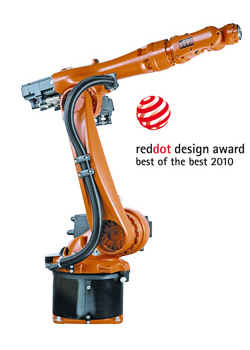
\includegraphics[width=0.45\textwidth]{PR_KR5_arc_02}
\caption{Robot KUKA KR5 Arc. Převzato z \cite{kuka_datasheet_url}.}
\label{kuka_kr5_pic}
\end{figure}

Tento robot s hmotností 127 kg a základní nosností 5 kg patří mezi lehčí průmyslové roboty. Byl vyvinut primárně pro aplikace vyžadující vysokou přesnost polohování, jako je obloukové svařování a přesná manipulace s lehkými pevnými předměty. Robot je schopen polohovat koncový efektor s přesností do 0,04 mm. Objem pracovní obálky je 8,4 \si{m^{3}}. Díky lehké konstrukci a výkonným pohonům o je robot schopen dosahovat vysokých provozních rychlostí s rychlostí koncového efektoru přesahující 5 \si{m/s}.  

\begin{figure}[ht]
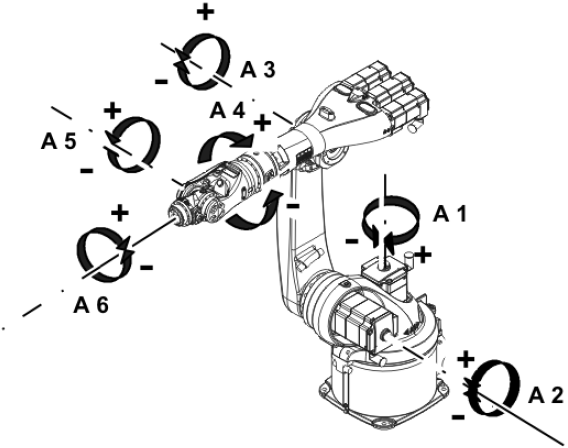
\includegraphics[width=0.65\textwidth]{kuka_kr5_axes}
\caption{Konfigurace os robota. Převzato z \cite{kuka_datasheet_url}.}
\label{kuka_kr5_axes_pic}
\end{figure}

Jako pohony os jsou použity třífázové synchronní servopohony s permanentními magnety (PMSM). Pro zvýšení točivého momentu motorů a přesnosti polohování jsou motory opatřeny převodovkou. Servomotory robota jsou vybaveny snímači pro snímání úhlu natočení rotoru, sondami pro měření proudu protékajícího jejich vinutím a tepelnými senzory pro měření teploty uvnitř motoru. Jednotlivé osy jsou dále vybaveny brzdným mechanismem, který zabraňuje otáčení os, pokud není robot v aktivním pohybu. 

Součástí robota je i řídící systém zajišťující napájení a řízení robota a poskytující uživatelské rozhraní (HMI) pro jeho programování a ovládání. Pohyb robota je programován v jazyce KRL (KUKA Robot Language). Součástí řídícího systému je i užitečný nástroj TRACE, umožňující sledování vnitřních stavů robota jako jsou polohy, rychlosti a zrychlení jednotlivých os, jejich momenty, protékající proudy a mnoho dalších. 

Celý systém je napájen z třífázové soustavy elektrické energie. Je určen pro montáž na zem nebo strop ve vnitřních prostorách. Podrobnější informace je možné nalézt v katalogovém listu. \cite{kuka_datasheet_url}.

%!TEX ROOT=ctutest.tex

\chapter{Dynamický model}

Pro výpočet a predikci spotřeby elektrické energie je nezbytné vytvořit matematický dynamický model robota. 

V případě 6-ti osového manipulátoru se jedná o systém se šesti stupni volnosti. K popisu jeho dynamiky je proto potřeba 6 rovnic druhého řádu. Celkově se tedy jedná o systém dvanáctého řádu. 

\section{Pohybové rovnice}
\label{pohybove_rovnice_sec}
K odvození pohybových rovnic je možné použít jeden ze dvou základních přístupů a to Newton-Eulerovu metodu nebo Euler-Lagrangeovu metodu. 

Newton-Eulerova metoda je založena na přístupu k systému jako k soustavě jednotlivých jeho částí a vyžaduje určení pohybových rovnic každé jednotlivé osy. Protože jsou jednotlivé osy vzájemně kinematicky propojeny, jsou i pohybové rovnice jednotlivých os závislé na pohybu ostatních os. 

Euler-Lagrangeova metoda naopak přistupuje k systému jako k celku a je založena na určení Lagrangianu, který je definován jako rozdíl jeho celkové kinetické a potenciální energie. Dynamické rovnice systému se poté odvodí vypočtením Lagrangeových rovnic druhého druhu pro všechny stupně volnosti.

Oba přístupy nakonec vedou ke stejným rovnicím. Protože jsou jednotlivé polohy a dynamika systému popisovány pomocí úhlů na jednotlivých osách, jsou tyto rovnice silně nelineární. V případě robota KR5 se jedná o soustavu 6 rovnic o celkem 24 neznámých (moment, poloha, rychlost a zrychlení pro každou osu). 

Rovnice systému je možné zapsat v následujícím maticovém tvaru jako 

\begin{equation}
T = M(\dot{\theta},\theta)\ddot{\theta} + C(\dot{\theta},\theta)\dot{\theta} + G(\theta)
\label{dyn_rovnice_eq}
\end{equation}

kde

\begin{description}
\item[$T = {\big[T_1  \dotsm  T_n\big]}^{T}$] je vektor momentů sil působících na jednotlivé osy robota
\item[$\ddot \theta = {\big[\ddot \theta_1  \dotsm  \ddot \theta_n\big]}^{T}$] je vektor úhlových zrychlení na jednotlivých osách
\item[$\dot \theta = {\big[\dot \theta_1  \dotsm  \dot \theta_n\big]}^{T}$] je vektor úhlových rychlostí na jednotlivých osách
\item[$M\big(\dot \theta, \theta\big)$] je matice setrvačnosti tvořena tenzory setrvačnosti jednotlivých os
\item[$C\big(\dot \theta, \theta\big)$] je matice Coriolisových a odstředivých momentů sil působících na jednotlivé osy
\item[$G\big(\theta\big)$] je matice gravitačních sil působících na jednotlivé osy
\item[$n$] je počet os
\end{description}

K výpočtu okamžité spotřeby elektrické energie je nutné řešit inverzní dynamickou úlohu, kdy se z okamžitých poloh, rychlostí a zrychlení na jednotlivých osách robota vypočítají točivé momenty, kterými působí motory. 

Moment síly motoru je závislý na proudu protékajícím jeho vinutím. Tuto závislost je často možné aproximovat lineární závislostí a psát jako
\begin{equation}
T\big(t\big) = KI\big(t\big)
\label{torque_current_eq}
\end{equation}

kde

\begin{description}
\item[$T\big(t\big) {\big[Nm\big]}$] je moment síly motoru 
\item[$K {\big[Nm/A\big]}$] je momentová konstanta 
\item[$I\big(t\big) {\big[A\big]}$] je proud protékající motorem 
\end{description}

Momentové konstanty jednotlivých motorů je možné zjistit v jejich dokumentaci. Nástroj TRACE robotu KUKA KR5 takto počítá momenty sil jednotlivých motorů. 

\section{Tření}

Odvozené rovnice dynamiky robota popsané výše v sekci \ref{pohybove_rovnice_sec} popisují pouze ideální model, ve kterém nedochází k žádným ztrátám energie. V reálných motorech a převodovkách ale dochází k energetickým ztrátám v důsledku tření v ložiscích motorů, rotačních os a tření v převodovkách.

Kompletní popis tření os je relativně komplikovaný. Proto se zpravidla pro jeho modelování používá zjednodušený model popisující tření jako kombinaci viskózního a Coulombova tření \cite{}. 

Viskózní tření je tření, které je lineárně závislé na rychlosti rotace. Při nulové rychlosti je třecí moment síly nulový a s rostoucí rychlostí se zvyšuje.

Coulombovo tření je naopak nezávislé na rychlosti rotace. V systému je přítomno vždy a se stejnou magnitudou. Mění se pouze se změnou směru otáčení, kdy mění znaménko.

Tento model je popsán rovnicí 

\begin{equation}
T_f = f_v\dot{\theta} + f_csign(\dot{\theta})
\label{fric_eq}
\end{equation}

kde

\begin{description}
\item[$T_f$] je moment síly generovaný třením 
\item[$f_v$] je koeficient viskózního tření 
\item[$f_c$] je koeficient coulombova tření 
\end{description}

Na následujícím obrázku (obr. \ref{treni_pic}) je znázorněn model tření včetně jeho jednotlivých složek. Na vodorovné ose je uvedena rychlost otáčení, na vertikální ose je třecí moment síly.

\begin{figure}[ht]
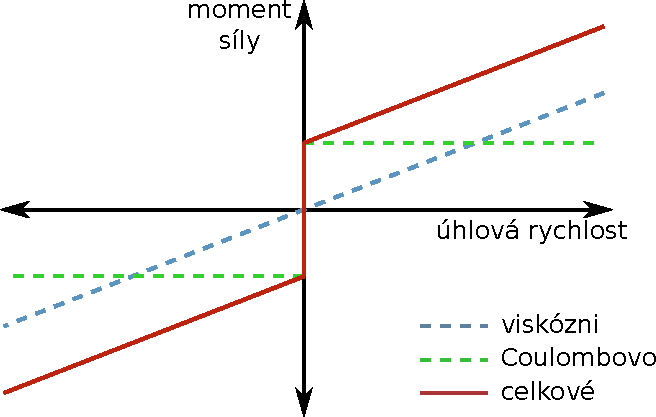
\includegraphics[width=0.65\textwidth]{treni}
\caption{Model tření os}
\label{treni_pic}
\end{figure}

Doplněním rovnice \ref{fric_eq} do dynamických rovnic robota \ref{dyn_rovnice_eq} se získají celkové rovnice dynamiky robota ve tvaru

\begin{equation}
T = M(\dot{\theta},\theta)\ddot{\theta} + C(\dot{\theta},\theta)\dot{\theta} + G(\theta) + F_v\dot{\theta} + F_csign(\dot{\theta})
\label{celkova_dyn_rovnice_eq}
\end{equation}

kde

\begin{description}
\item[$F_v$] je vektor koeficientů viskózního tření v jednotlivých osách
\item[$F_c$] je vektor koeficientů Coulombova suchého tření v jednotlivých osách
\end{description}

\section{Elektrický výkon}

Výkon je obecně definován jako práce vykonaná za jednotku času a platí rovnice

\begin{equation}
P = \frac{W}{t}
\end{equation}

Protože v tomto případě se jedná o elektrickou práci, je tato práce definovaná jako celkový náboj $q$ přenesený mezi dvěma místy s napětím $u$. Platí tedy vztah

\begin{equation}
P = \frac{uq}{t}
\end{equation}

Pro okamžitý výkon je poté možné tento vzorec upravit na

\begin{equation}
p(t) = u(t)\frac{dq}{dt} = u(t)i(t)
\end{equation}

\subsection{Elektrický výkon v třífázové soustavě}

V případě harmonického střídavého napětí a proudu platí

\begin{equation}
\begin{split}
u\big(t\big) = U_m cos\big(\omega t + \phi\big) \\
i\big(t\big) = I_m cos\big(\omega t + \phi + \psi\big)
\end{split}
\label{harm_curr_volt_eq}
\end{equation}  
kde
\begin{description}
\item[$U_m$] je maximální amplituda napětí
\item[$I_m$] je maximální amplituda proudu
\item[$\omega$] je úhlová frekvence
\item[$\phi$] je počáteční fáze proudu a napětí
\item[$\psi$] je fázový posun mezi napětím a proudem
\end{description}

Pokud je fázový posun $\psi$ mezi napětím a proudem nenulový, je potřeba rozdělit elektrický výkon na činnou a jalovou složku. Činná složka výkonu je výkon, který je přenášen ze zdroje do spotřebiče a který je schopen konat práci. Pro činnou složku výkonu platí následující vztah

\begin{equation}
P = \frac{1}{T} \int_{t_0}^{t_0 + T} p(t)dt = UI cos\phi
\label{act_power_eq}
\end{equation}  

kde $U$ je efektivní hodnota napětí a $I$ je efektivní hodnota proudu.

Jalová složka výkonu je část výkonu, která je spotřebičem vracená zpět do zdroje a ve spotřebiči tedy žádnou práci nevykonává.

V případě třífázové soustavy je její celkový výkon roven součtu výkonů v jednotlivých fázích. Platí tedy

\begin{equation}
P = P_U + P_V + P_W
\label{3ph_power_eq}
\end{equation}  

kde $U,V,W$ jsou jednotlivé fáze v třífázové soustavě.

\subsection{Elektrický výkon synchronního motoru}

V případě výpočtu výkonu elektrického motoru je potřeba vytvořit model jeho vinutí. Synchronní motor s permanentními magnety je možné zjednodušeně modelovat jako stejnosměrný (DC) motor. Jeho elektrické schéma je na obrázku \ref{schema_motoru_pic}.  

\begin{figure}[ht]
\includegraphics[width=0.55\textwidth]{obvod_motoru}
\caption{Elektrické schéma vinutí synchronního motoru.}
\label{schema_motoru_pic}
\end{figure}

$R$ je vnitřní elektrický odpor vinutí a $L$ je jeho indukčnost. Tyto hodnoty jsou zpravidla udávány v datasheetech k motorům.

Pro okamžité napětí $u(t)$ ze schématu platí 

\begin{equation}
u(t) = i(t)R + L\frac{di(t)}{dt}
\label{motor_voltage_eq}
\end{equation}  

Okamžitý elektrický výkon motoru je poté možné z měření okamžité efektivní hodnoty proudu vypočítat jako
 
\begin{equation}
p(t) = i(t)u(t) = i(t)\left(i(t)R + L\frac{di(t)}{dt}\right)
\label{motor_power_eq}
\end{equation} 

Celkový okamžitý elektrický výkon při pohybu robota je poté dán jako součet okamžitých výkonů na všech jeho motorech
\begin{equation}
P(t) = \sum_{i=1}^{n} p_i(t)
\label{robot_motor_power_eq}
\end{equation} 
kde $n$ je počet motorů.

\section{Solver ReDySim}

Pro usnadnění odvození soustavy rovnic pro robota o 6 stupních volnosti a pro případnou standardizaci metody pro použití i pro jiné typy robotů byl použit skript pro matematický nástroj MATLAB využívající solver Recursive Dynamic Simulator (ReDySim)\cite{redysim}. Tento nástroj byl vyvinut na univerzitě v Dillí a je bezplatně k dispozici ke stažení a použití v MATLABu. Je schopen generovat rovnice pro libovolný počet os a to jak pro rotační, tak lineární osy. 

Jeho vstupními parametry jsou modifikované DH (Denavit-Hartenbergovy) parametry robota a dynamické parametry s numerickými nebo symbolickými hodnotami. Výstupem je poté skript pro MATLAB s vygenerovanými pohybovými rovnicemi zadaného robota.  

\section{Modifikované DH parametry robota}

Modifikované Denavit-Hartenbergovy (DH) parametry jsou parametry, pomocí nichž je možné kompletně popsat geometrii a kinematiku sériového robota. Jedná se o čtyři parametry pro každou osu robota, které definují vzájemnou polohu a konfiguraci sousedících os. 

Parametr $a_i [m]$ popisuje délku ramena $i$, $b_i [m]$ udává odsazení ramena $i$ podél osy rotace ramena $i-1$, parametr $\alpha_i [\si{\degree}]$ určuje vzájemný úhel natočení mezi osou $i+1$ a osou $i$ a poslední parametr $\theta_i [\si{\degree}]$ udává okamžitý úhel natočení osy $i$.

V tabulce č.\ref{tab_DH_kuka} je DH parametrizace robota KUKA KR5 Arc použita v nástroji ReDySim.

\begin{table}[htbp]
  \centering
  \caption{Tabulka DH parametrů KUKA KR5 Arc.}
    \begin{tabular}{c|cccccccccc}
    \multicolumn{1}{c|}{Osa} & \multicolumn{1}{c}{$a_{i} [m]$} & \multicolumn{1}{c}{$b_{i} [m]$} & \multicolumn{1}{c}{$\alpha_{i} [\si{\degree}]$} \\
    \hline
    1     &   0.18  &  0.4   &  90     &     \\
    2     &   0.6   &  0     &  180    &     \\
    3     &   0.12  &  0     &  -90    &     \\
    4     &   0     &  0.62  &  -90    &     \\
    5     &   0     &  0     &  90     &     \\
    6     &   0     &  0.115 &  0      &     \\
    \end{tabular}%
  \label{tab_DH_kuka}%
\end{table}% 

Přesné délky jednotlivých ramen a vzájemné polohy jednotlivých os robota je možné nalézt v jeho dokumentaci.

Pro vizualizaci DH parametrizace je možné použít nástroj RoboAnalyzer [\cite{roboanalyzer}], který byl vyvinut společně se solverem ReDySim pro účely vizualizace a simulace. RoboAnalyzer umožňuje simulovat jednoduché pohyby robota s až 7 osami a vykreslovat průběhy stavů jako jsou polohy, rychlosti, zrychlení a momenty sil na jednotlivých osách. Vizualizace použité DH parametrizace pro robota KUKA KR5 Arc v prostředí RoboAnalyzer je na obrázku \ref{dh_kuka_pic}.
\\
\begin{figure}[ht]
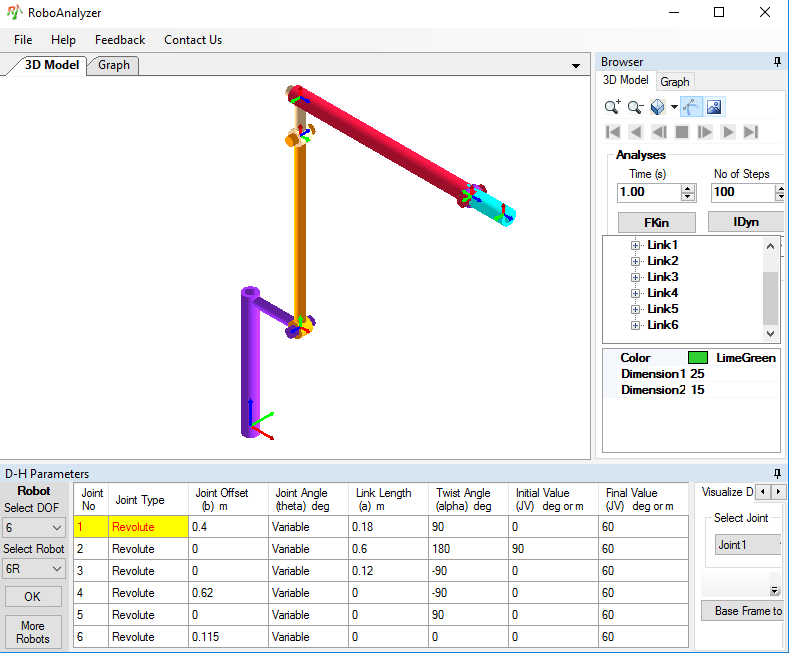
\includegraphics[width=0.95\textwidth]{pic_dh_kuka}
\caption{Vizualizace DH parametrizace robota KUKA KR5 Arc.}
\label{dh_kuka_pic}
\end{figure}



%!TEX ROOT=ctutest.tex

\chapter{Identifikace systému}

U robotického manipulátoru zpravidla nejsou zcela známy informace o dynamických parametrech robota, jako jsou momenty setrvačnosti, hmotnosti nebo koeficienty tření jednotlivých os. Tyto informace nejsou v běžných situacích poskytovány ani samotnými výrobci robotů. Je to hlavně proto, že pro zákazníka nejsou tyto údaje důležité, protože se robotické manipulátory dodávají jako hotové uzavřené systémy připravené k použití a jejich řízení je již výrobcem implementováno v jejich řídicím systému.

\section{Způsoby identifikace}

Protože obvykle nejsou známy všechny dynamické parametry, je pro vytvoření dynamického modelu nutné tyto parametry nějakým způsobem získat nebo odvodit. Toho je možné docílit několika způsoby.

\subsection{Z přímého měření součástí robota}

Dynamické parametry je možné určit rozebráním robota na menší součásti a přímým měřením jejich dynamických vlastností. Tento způsob se jeví jako nejpřirozenější.

Určení parametrů takovýmto způsobem je ale možné pouze u jednoduchých laboratorních modelů robota tvořených malým počtem součástí. U větších a složitějších robotů, jako jsou průmyslové manipulátory, je tento způsob náročný časově i způsobem provedení. Jednotlivá ramena sestávají z více komponent, jako jsou samotné kostry ramen, převodovky motorů, napájecí a komunikační vedení motorů a dalších. Ty mohou dále sestávat z dalších součástek. Rozebrání robota navíc může způsobit ztrátu podpory a záruky ze strany výrobce.

Další nevýhodou je nemožnost zobecnění tohoto způsobu na více typů robotů. Každý nový typ robota by se musel rozebrat a změřit, i kdyby se jednalo o robota podobného typu a konstrukce. Proto se tato práce tímto postupem dále nezabývá.    

\subsection{Z 3D modelu}

Výrobci často poskytují ke stažení 3D modely svých robotů. Obvykle tyto modely slouží pro účely vytvoření počítačových simulací nebo modelů výrobních linek. 
3D modely je možné použít ke zjištění neznámých dynamických parametrů jejich analýzou v nástrojích CAD, jako je například AutoCAD nebo Siemens NX. Tyto nástroje jsou schopny z geometrie objektů počítat jejich objemy, momenty setrvačnosti, polohy těžišť a hmotnosti.

Výhodou tohoto postupu je jeho rychlost a jednoduchost. Navíc je takto možné získat požadované parametry i bez nutnosti přístupu k opravdovému fyzickému robotu. Tento postup je také možné zobecnit na libovolný typ robotického manipulátoru. Stačí k němu jen mít jeho odpovídající 3D model. 3D model robotu KUKA KR5 Arc v prostředí Siemens NX 10.0 je na obrázku \ref{kuka_3d_pic}.

\begin{figure}[ht]
    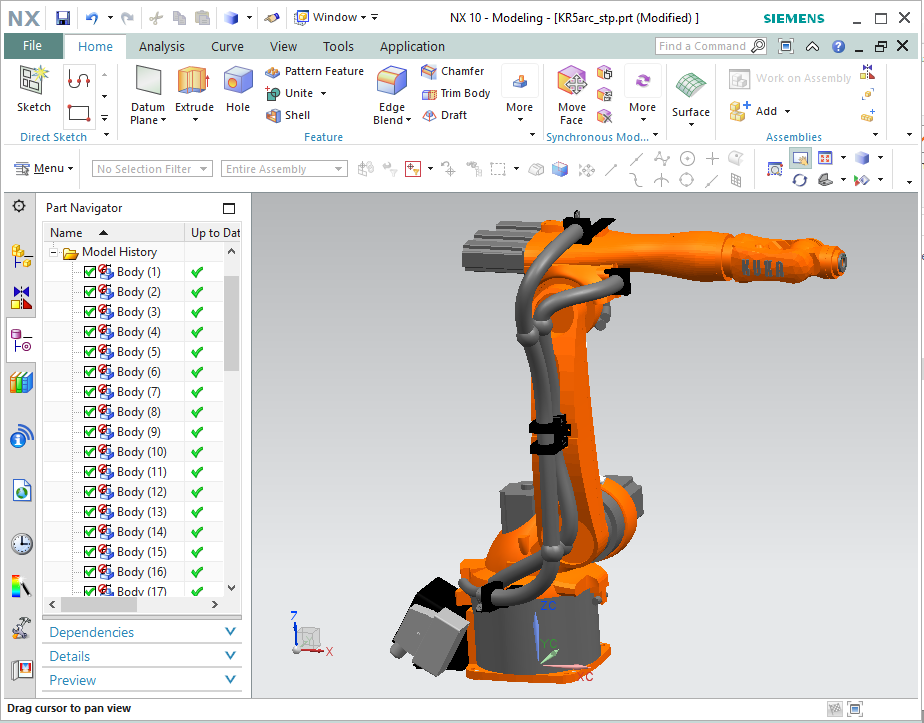
\includegraphics[width=0.8\textwidth]{kuka_3d}
    \caption{3D model robotu KUKA KR5 Arc v prostředí Siemens NX 10.0.}
    \label{kuka_3d_pic}
\end{figure}

3D model ale zpravidla popisuje pouze povrchovou geometrii jednotlivých komponent robota a neobsahuje informace o jejich vnitřní konstrukci, typech použitých materiálů, jejich skutečných hmotnostech nebo hustotách. Je zde možnost považovat jednotlivé součásti robotu za tělesa s homogenní hustotou a hmotnosti odhadnout z celkové hmotnosti robotu, která bývá udávána v jeho datasheetu. Tento postup ale dává jen velmi hrubý odhad dynamických parametrů. 

Navíc z 3D modelu není možné získat informace o koeficientech tření v jednotlivých osách. 

Tento způsob identifikace je v této práci použit pouze pro účely porovnání určených hodnot s hodnotami odvozenými metodou popsanou v sekci \ref{z_rovnic_sec}.
\label{z_3d_modelu_sec}

\subsection{Z rovnic}
\label{z_rovnic_sec}
Neznámé dynamické parametry je možné přesně vypočítat pomocí dynamických rovnic robota. 

Přestože jsou dynamické rovnice robota \ref{celkova_dyn_rovnice_eq} nelineární vůči jednotlivým zobecněným souřadnicím, jsou lineární vůči jednotlivým složkám dynamických parametrů [\cite{clos_dyn_par}][\cite{dyn_mod_ind}]. Proto je tyto rovnice možné je přepsat do tvaru

\begin{equation}
T(t) = H(\ddot{\theta}(t),\dot{\theta}(t),\theta(t))P
\label{eq_lin_par}
\end{equation}
kde
\begin{description}
\item[$T(t) = {\big[T_1(t)  \dotsm  T_n(t)\big]}^{T}$] je vektor momentů sil na osách v čase $t$ 
\item[$P = {\big[P_1  \dotsm  P_n\big]}^{T}$] je vektor neznámých dyn. parametrů jednotlivých os
\item[$n$] je počet os
\end{description} \noindent
a \ \ \ \ \ \ $P_i = {\big[I_{ixx} \ I_{ixy} \ I_{iyy} \ I_{iyz} \ I_{izz} \ I_{izx} \ m_i \ m_id_{ix} \ m_id_{iy} \ m_id_{iz} \ f_{vi} \ f_{ci}\big]}^{T}$ \\
\\
\\
kde
\noindent
\begin{description}
\item[$I_{ijk}$] je složka setrvačnosti pro link $i$ vůči souřadnicím $j$ a $k$
\item[$r_{ij}$] je složka vektoru těžiště linku $i$ vyjádřená v souřadnici $j$
\item[$m_{i}$] je hmotnost linku $i$
\item[$f_{vi}$] je koeficient viskózního tření linku $i$
\item[$f_{ci}$] je koeficient Coulombova tření linku $i$
\end{description}

Počet neznámých parametrů pro jedno rameno robotu odpovídá počtu složek vektoru $P_i$. Ten je roven 12. U sériového průmyslového manipulátoru se šesti rotačními osami je tedy neznámých parametrů celkem 72. 

Počet neznámých parametrů je možné zredukovat. Je to možné díky tomu, že některé parametry dynamiku robota neovlivní nebo je jejich vliv zanedbatelný. Důvodem je to, že se některé linky mohou otáčet pouze kolem některé z os. Příkladem může být osa 1 (spojená se zemí, viz schéma \ref{kuka_kr5_axes_pic}), která se v prostoru může otáčet jen kolem vertikální osy. Tím je možné zanedbat momenty setrvačnosti mimo tuto vertikální osu. Dále je možné zanedbat její hmotnost a polohu jejího těžiště. Zároveň je možné model dále zjednodušit uvažováním pouze prvků na hlavní diagonále tenzorů setrvačnosti a zanedbáním prvků mimo ni.

Díky tomu klesne počet neznámých parametrů v případě šestiosového robotu z čísla 72 na číslo 48. V následující tabulce (tabulka \ref{tab_hled_param}) je přehled výsledných neznámých dynamických parametrů robota KUKA KR5 Arc.
\\

\begin{table}[ht]
  \centering
  \caption{Tabulka nezámých parametrů robota KUKA KR5 Arc.}
    \begin{tabular}{c|lllllllll}
    \multicolumn{1}{c|}{Osa} & \multicolumn{9}{c}{Neznámé parametry}  \\
    \hline
    1 &       	  &	          & $I_{1zz}$ &          &          &          & & $f_{v1}$ & $f_{c1}$ \\
    2 & $I_{2xx}$ & $I_{2yy}$ & $I_{2zz}$ & $d_{2x}$ & $d_{2y}$ & $d_{2z}$ & $m_{2}$ & $f_{v2}$ & $f_{c2}$ \\
    3 & $I_{3xx}$ & $I_{3yy}$ & $I_{3zz}$ & $d_{3x}$ & $d_{3y}$ & $d_{3z}$ & $m_{3}$ & $f_{v3}$ & $f_{c3}$ \\
    4 & $I_{4xx}$ & $I_{4yy}$ & $I_{4zz}$ & $d_{4x}$ & $d_{4y}$ & $d_{4z}$ & $m_{4}$ & $f_{v4}$ & $f_{c4}$ \\
    5 & $I_{5xx}$ & $I_{5yy}$ & $I_{5zz}$ & $d_{5x}$ & $d_{5y}$ & $d_{5z}$ & $m_{5}$ & $f_{v5}$ & $f_{c5}$ \\
    6 & $I_{6xx}$ & $I_{6yy}$ & $I_{6zz}$ & $d_{6x}$ & $d_{6y}$ & $d_{6z}$ & $m_{6}$ & $f_{v6}$ & $f_{c6}$ \\
    \end{tabular}%
  \label{tab_hled_param}%
\end{table}%

Hledané parametry je poté možné vypočítat z rovnice \ref{eq_lin_par} jejich vyjádřením ve tvaru

\begin{equation}
P = H\big(\ddot{\theta}(t),\dot{\theta}(t),\theta(t)\big)^{-1}T(t)
\label{eq_lin_par_inv}
\end{equation}

K výpočtu vektoru $P$ neznámých parametrů je nejprve potřebné s robotem vykonat pohyb po nějaké trajektorii a měřit polohy, úhlové rychlostí, úhlová zrychlení a momenty sil na jednotlivých osách. Do matice $H\big(\ddot{\theta}(t),\dot{\theta}(t),\theta(t)\big)$ se poté dosadí tyto změřené polohy, úhlové rychlosti a úhlová zrychlení jednotlivých os v čase $t$ a do vektoru $T(t)$ změřené momenty sil v čase $t$. 

Protože je ale neznámých parametrů více než rovnic, nelze tuto rovnici vyřešit jednoznačně. Tento problém lze jednoduše vyřešit naměřením více bodů na trajektorii v různých časech a jejich následným dosazením do rovnice \ref{eq_lin_par_inv}. Důležité je na trajektorii mít změřen takový počet bodů, aby z této rovnice vznikla rovnice přeurčená. Takovou přeurčenou rovnici je poté možné řešit například použitím metody nejmenších čtverců, která minimalizuje střední odchylku mezi skutečnými a odhadnutými parametry a navíc je schopna eliminovat vliv šumu měření. 

\subsection{Excitační trajektorie}

Neznámé parametry identifikované postupem popsaným v sekci \ref{eq_lin_par} jsou silně závislé na zvolené trajektorii, na které jsou měřeny průběhy dynamických veličin. 

Aby tímto způsobem bylo možné správně odhadnout hodnoty všech neznámých parametrů, je potřeba s robotem vykonat pohyby po takové trajektorii, na které by byly vybuzeny všechny dynamické složky robota. Trajektorie musí být zvolena tak, aby se do dynamiky pohybu promítly všechny neznámé parametry. Identifikace z nedostatečně budící (excitující) trajektorie sice také odhadne všechny neznámé parametry, model s nimi ale bude přesný pouze pro pohyby po této trajektorii nebo jejím okolí.

Ve vědeckých článcích a publikacích např. \cite{dyn_mod_ind}\cite{dyn_ind_mits}\cite{clos_dyn_par} se na jednotlivých osách jako excitační trajektorie doporučují trajektorie, které je možné popsat konečnou Fourierovou řadou. Jejich výhodou je, že díky vlastnostem harmonických funkcí jsou poté jednotlivé polohy, rychlosti i zrychlení rovněž kombinací harmonických průběhů. Tím je maximalizován vliv hledaných dynamických parametrů a minimalizován vliv šumu měření. 

Protože se průmyslové manipulátory používají převážně pro polohování, jejich řídicí systémy zpravidla neumožňují na osách provádět čistě harmonické průběhy. Řídicí systém robota KUKA KR5 Arc umožňuje zadat požadovanou trajektorii dvěma hlavními způsoby. První způsob je zadání trajektorie jako sady požadovaných poloh os, kterých musí osy dosáhnout a rychlosti/zrychlení, s jakými se má tento pohyb vykonat. Druhou možností je zadání požadovaných poloh a rychlostí koncového efektoru v kartézských souřadnicích. Řídicí systém následně sám tyto zadané polohy aproximuje hladkou trajektorií. 

Z tohoto důvodu je nutné robotu poskytnout sérii bodů popisujících harmonický průběh. Výsledná trajektorie robota je poté pouze aproximací harmonického průběhu.  

\section{Postup identifikace}

Při identifikaci parametrů robota KUKA KR5 Arc se postupovalo způsobem popsaným výše v sekci \ref{z_rovnic_sec}. 

Pomocí nástroje ReDySim byla vygenerována soustava šesti rovnic dynamiky robota. Protože ReDySim v rovnicích neuvažuje tření na jednotlivých osách, bylo nutné toto tření do vygenerovaných rovnic ručně doplnit. Výsledná soustava rovnic se poté převedla do maticového tvaru lineárního vůči neznámým dynamickým parametrům (rovnice \ref{eq_lin_par}). 

Za vektor $P$ neznámých parametrů byl zvolen vektor s parametry všech šesti os
\[\addtolength{\arraycolsep}{-1.5pt}
\begin{split}
P &= 
[\begin{matrix} I_{1x} & I_{1y} & I_{1z} &\cdots &I_{6x} & I_{6y} & I_{6z} \end{matrix} \\
 &\qquad\qquad \begin{matrix}  m_1 & m_1d_{1x} & m_1d_{1y} & m_1d_{1z} &\cdots & m_6 & m_6d_{6x} & m_6d_{6y} & m_6d_{6z} \end{matrix} \\
 &\qquad\qquad\qquad\qquad \begin{matrix} f_{v1} & f_{c1} &\cdots & f_{v6} & f_{c6} \end{matrix}]^{T}
\end{split}
\]

Do matic $H\big(\ddot{\theta}(t),\dot{\theta}(t),\theta(t)\big)$ a $T(t)$ se dosadily jednotlivé polohy os, úhlové rychlosti, úhlová zrychlení a momenty sil naměřené v různých časech na identifikační trajektorii. Vektor neznámých parametrů $P$ se poté vypočítal z rovnice \ref{eq_lin_par_inv} metodou nejmenších čtverců. 

Protože jsou dynamické rovnice robota silně nelineární, může se stát, že řešitel metody nejmenších čtverců nenalezne globálně optimální řešení, ale skončí v některém z lokálních minim. Je také možné, že řešitel nalezne řešení, které bude správně matematicky, fyzikálně ale nebude dávat smysl (záporné hmotnosti ramen, apod.). Z tohoto důvodu je vhodné nějakým způsobem omezit prostor, ve kterém se má řešení hledat.

V této práci byl pro řešení metody nejmenších čtverců v MATLABu použit solver \texttt{lsqlin}, který umožňuje specifikovat hranice, ve kterých se má hledat řešení. První z omezujících podmínek bylo, že všechny hmotnosti a momenty setrvačnosti mají mít kladné hodnoty. Dále se nastavilo omezení na hledané polohy těžiště ramen tak, aby tato těžiště neležela mimo fyzický objem ramen. Posledním z požadovaných omezení bylo nastavení přesných hmotností ramen, které bylo možné dohledat ve zdrojových datech robotu.

\label{postup_identifikace_ch}

\subsection{Identifikační trajektorie}

Protože je prostor kolem robotu omezen, není možné s robotem provádět pohyby v jeho plném rozsahu. Proto tomu bylo nutné přizpůsobit identifikační trajektorii. Identifikační trajektorie byla vytvořena složením několika nezávislých trajektorií. 

V první části trajektorie se pohybovalo pouze s posledními třemi osami (osa 6, osa 5 a osa 4). Ostatní osy byly v pevně zafixované pozici. Nejprve se opakovaně pohybovalo pouze poslední šestou osou v jejím maximálním možném rozsahu v obou směrech otáčení. K tomu se následně přidal obdobný pohyb páté osy a nakonec se stejným způsobem přidal i pohyb čtvrté osy. Tímto se pokryla maximální možná škála pohybů posledních tří os.

Následovala část trajektorie pro identifikaci parametrů prvních tří os. U těchto os je situace zkomplikovaná tím, že osa 2 a osa 3 mají vždy vzájemně rovnoběžné osy otáčení (viz obrázek \ref{kuka_kr5_axes_pic}). Proto je obtížné nezávisle identifikovat některé z jejich parametrů. Příkladem může být identifikace momentů setrvačnosti vzhledem k osám kolmým na osy jejich rotace. Osou 3 není možné kolem těchto os otáčet, aniž by se zároveň kolem stejné osy neotáčela osa 2 a naopak.    

V tomto případě se postupovalo nejprve opakovaným pohybem osy 3 v jejím plném rozsahu a zafixováním os 1 a 2. Následně se zafixovala osa 3 a stejným způsobem se pohybovalo osou 2. Tímto se pokryly pohyby nezávislé na rotaci kolem osy 1. 

Trajektorie závislá na pohybu osy 1 byla vytvořena tak, že se nejprve několikrát pohybovalo osou 1 s rameny os 2 a 3 pevně zafixovanými ve vertikální poloze. Poté se stejné pohyby provedly s ramenem osy 3 v horizontální poloze a následně s oběma rameny 2 a 3 v horizontální poloze.

Výsledná identifikační trajektorie byla vytvořena spojením těchto tří trajektorií v jednu. Nástroj TRACE přitom byl nastaven tak, aby prováděl měření poloh, úhlových rychlostí, úhlových zrychlení, momentů sil a proudů na všech osách. 

\section{Skript pro MATLAB}

Pro účely identifikace robota KUKA KR5 Arc byl vytvořen skript pro použití v MATLABu, který umožňuje vytvoření dynamického modelu, načtení změřených trajektorií, identifikaci neznámých parametrů, simulaci a srovnání výsledků a analýzu vlivu nepřesnosti odhadnutých parametrů na přesnost modelu.

Skript je rozdělen na několik po sobě jdoucích podprogramů, které je možné spouštět vcelku nebo po jednotlivých částech. Komentáře ve skriptu jsou psány v anglickém jazyce pro případné rozšíření jeho použití.

První část je univerzální pro libovolného sériového robota s rotačními osami. Definují se zde základní parametry robotu, jako je počet os, délky jednotlivých ramen, převodní poměry převodovek a počet měřených veličin. Dále se zde zadávají parametry motorů, mezi něž patří momentové konstanty a odpory a indukčnosti vinutí. 

Další část je částečně závislá na použitém robotu. V této části je importována změřená trajektorie robota. Robot KUKA KR5 Arc používá k měření trajektorií nástroj TRACE. Tento nástroj ukládá změřená data ve speciální struktuře ve formátu .r64. Tu je potřeba rozložit na jednotlivé měřené složky a ty dále vynásobit převodními koeficienty měření. Jiné typy robotů, obzvláště roboty od jiných výrobců budou pravděpodobně mít změřené trajektorie ukládány jiným způsobem a v jiných formátech. Proto je potřeba, v případě použití jiného robotu, skript upravit nebo doplnit pro správné importování těchto dat. Výsledkem této části je trojrozměrná matice naměřených trajektorií pro jednotlivé osy a veličiny. 

Následující části jsou již zcela nezávislé na robotické platformě a jsou univerzální pro použití pro libovolného robota.  

Nejprve je vytvořen vektor $P$ parametrů v symbolickém tvaru. Následuje načtení vygenerovaných rovnic z nástroje ReDySim, jejich převod do symbolického tvaru a uložení do matice rovnic. Z té je poté vygenerovaná matice $H_i\big(\ddot{\theta}(t),\dot{\theta}(t),\theta(t)\big)$ se symbolickými proměnnými, do kterých je možné dosazovat změřená data.

Postupným dosazováním naměřených bodů na trajektorii (polohy, úhlové rychlosti a úhlová zrychlení) do matice $H_t\big(\ddot{\theta}(t),\dot{\theta}(t),\theta(t)\big)$ je vytvořena matice $H$. Současně je vytvořen vektor $T$ s dosazenými změřenými momenty sil.

Tyto vektory a matice jsou poté předány solveru \texttt{lsqlin}, který vypočte vektor $P$ vyřešením rovnice \ref{eq_lin_par_inv} metodou nejmenších čtverců. Zároveň je zde možné nastavit horní i spodní hranice jednotlivých parametrů vektoru $P$ ve kterých má solver řešení hledat.

Model s odvozenými parametry je možné v další části hned odsimulovat a porovnat se skutečnými změřenými trajektoriemi.

V poslední části je provedena analýza vlivu odchylek v hodnotách parametrů na přesnost energetického modelu robotu. Analýza vlivu odchylek je provedena pomocí metody Monte Carlo. Model je v cyklu odsimulován 200 krát pokaždé s jinou náhodně vygenerovanou hodnotou přičtenou k parametru. Poté je vypočítána střední odchylka mezi simulací a měřením. Tento postup je v cyklu opakován pro všechny identifikované parametry. 

Následuje vyhodnocení těchto výsledku a nalezení případů, kdy byla odchylka mezi modelem a změřenými hodnotami největší. Ve skriptu je možné upravovat počet simulací a rozsah odchylek parametrů.  



%!TEX ROOT=ctutest.tex

\chapter{Identifikované parametry}

Postupem popsaným v sekci \ref{postup_identifikace_ch} se podařilo identifikovat všechny neznámé parametry. Identifikované parametry jsou uvedeny v tabulce \ref{tab_ind_hodnot}. V následující tabulce \ref{tab_ind_hodnot_3d} jsou pro srovnání vypsané hodnoty identifikované z 3D modelu robota (viz sekce \ref{z_3d_modelu_sec}). Hodnoty v tabulkách jsou uvedeny v základních jednotkách SI. 
\\
\begin{table}[htbp]
  \centering
  \caption{Tabulka identifikovaných parametrů z rovnic}
    \begin{tabular}{c|cccccccccc}
    \multicolumn{1}{c|}{Osa} & \multicolumn{1}{c}{$I_{xx}$} & \multicolumn{1}{c}{$I_{yy}$} & \multicolumn{1}{c}{$I_{zz}$} & \multicolumn{1}{c}{$d_x$} & \multicolumn{1}{c}{$d_y$} & \multicolumn{1}{c}{$d_z$} & \multicolumn{1}{c}{$m$} & \multicolumn{1}{c}{$f_v$} & \multicolumn{1}{c}{$f_c$} \\
    \hline
    1  & 0     & 0     & 3.963 & 0     & 0     & 0     & 0     & 93.540 &  6.473 \\
    2  & 0.197 & 3.078 & 1.967 & 0.301 & 0.034 & 0     & 19.30 & 93.240 & 21.107 \\
    3  & 0.490 & 3.025 & 0.799 &-0.038 &-0.133 &-0.006 & 26.47 & 24.510 &  2.486 \\
    4  & 1.737 & 0.509 & 0.637 &-0.037 & 0.024 &-0.027 & 7.41  &  7.235 &  1.594 \\
    5  & 0.105 & 0.353 & 0.218 & 0.030 & 0     &-0.140 & 2.53  &  1.863 &  1.033 \\
    6  & 0.179 & 0.206 & 0.027 & 0     & 0     & 0.133 & 0.60  &  1.148 &  0.396 \\
    \end{tabular}%
  \label{tab_ind_hodnot}%
\end{table}%

\begin{table}[htbp]
  \centering
  \caption{Tabulka identifikovaných parametrů z 3D modelu}
    \begin{tabular}{c|cccccccccc}
    \multicolumn{1}{c|}{Osa} & \multicolumn{1}{c}{$I_{xx}$} & \multicolumn{1}{c}{$I_{yy}$} & \multicolumn{1}{c}{$I_{zz}$} & \multicolumn{1}{c}{$d_x$} & \multicolumn{1}{c}{$d_y$} & \multicolumn{1}{c}{$d_z$} & \multicolumn{1}{c}{$m$} & \multicolumn{1}{c}{$f_v$} & \multicolumn{1}{c}{$f_c$} \\
    \hline
    1  & 0.322   & 0.467   & 0.478   & 0.091 & 0.067 & 0.006 & 26.98 & - & - \\
    2  & 0.541   & 0.552   & 0.044   & 0.333 & 0.002 & 0.039 & 15.92 & - & - \\
    3  & 0.775   & 0.750   & 0.210   &-0.032 &-0.008 &-0.034 & 25.85 & - & - \\
    4  & 0.010   & 0.020   & 0.024   & 0     & 0.109 &-0.008 & 4.09  & - & - \\
    5  & 0.002   & 0.004   & 0.004   & 0     &-0.01  & 0     & 1.62  & - & - \\
    6  & 0.00006 & 0.00003 & 0.00003 & 0     & 0     & 0.111 & 0.02  & - & - \\
    \end{tabular}%
  \label{tab_ind_hodnot_3d}%
\end{table}%

Porovnáním hodnot v obou tabulkách je patrné, že se většina parametrů, snad jen s výjimkou hmotností ramen, poměrně výrazně liší. Dalším rozdílem je, že z 3D modelu není možné získat informace o koeficientech tření v jednotlivých osách, zatímco odvození z rovnic s třením počítá. Jak bude patrné ze simulace odvozených parametrů, tření má na dynamiku nezanedbatelný vliv.

\section{Simulace odvozených parametrů}

Na následujících obrázcích (obr. \ref{osa_1_sim_pic} až \ref{osa_6_sim_pic}) jsou odsimulované průběhy točivých momentů s odvozenými parametry všech šesti os. Jsou v nich odsimulované průběhy s parametry odvozenými pomocí rovnic a z 3D modelu. Ty jsou srovnány se skutečnými naměřenými momenty sil. 

Protože z 3D modelu není možné získat koeficienty tření os, je zde možnost uvažovat tyto koeficienty jako nulové a tím je v modelu zanedbat. Tento model je ale velmi nepřesný (viz průběhy níže). Na průbězích je vidět, že vychází opravdu velmi vysoké odchylky od naměřených dat. Tření os hraje v dynamice robota významnou roli, proto ho není možné tímto způsobem zanedbat.

Odvozené parametry z 3D modelu je možné využít tak, že se budou v dynamických rovnicích uvažovat jako známé a z rovnic se odvodí pouze neznámé koeficienty tření. Na průbězích níže jsou pro srovnání odsimulované průběhy s parametry získanými tímto způsobem. 

\hfill
\begin{figure}[h]
    \centering
    \begin{subfigure}[b]{1\textwidth}
        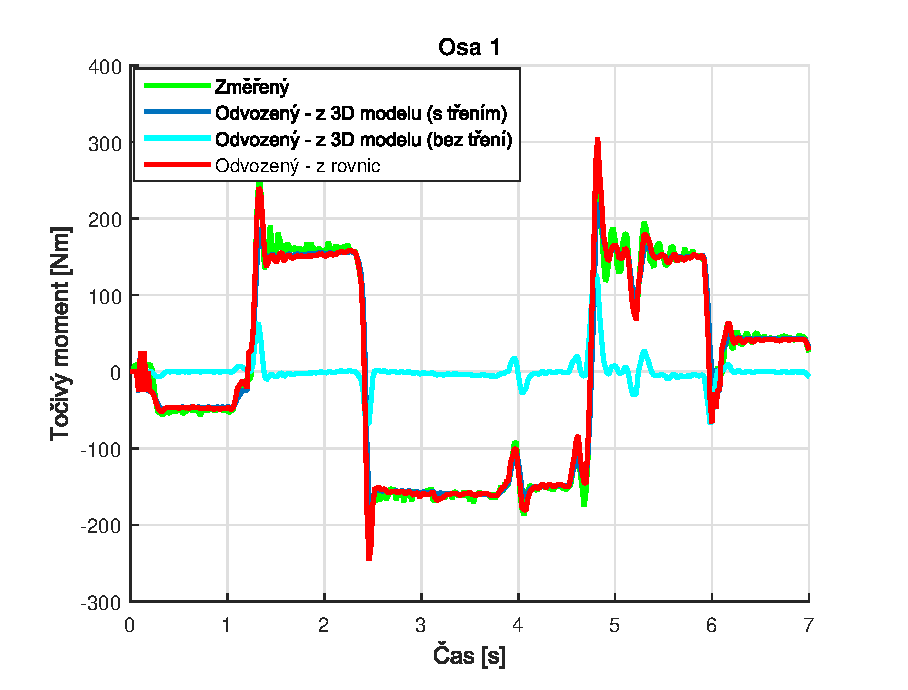
\includegraphics[width=\textwidth]{Osa_1_sim}
        \caption{Osa 1}
        \label{osa_1_sim_pic}
        \end{subfigure}
\end{figure}
\begin{figure}\ContinuedFloat    
    \begin{subfigure}[b]{1\textwidth}
        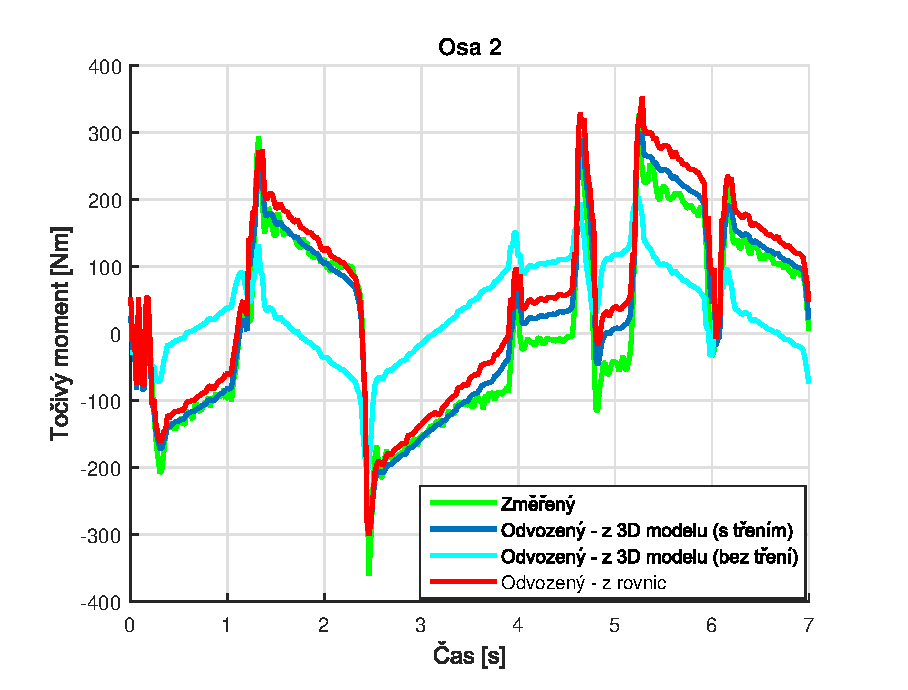
\includegraphics[width=\textwidth]{Osa_2_sim}
        \caption{Osa 2}
        \label{osa_2_sim_pic}
    \end{subfigure}
    \begin{subfigure}[b]{1\textwidth}
        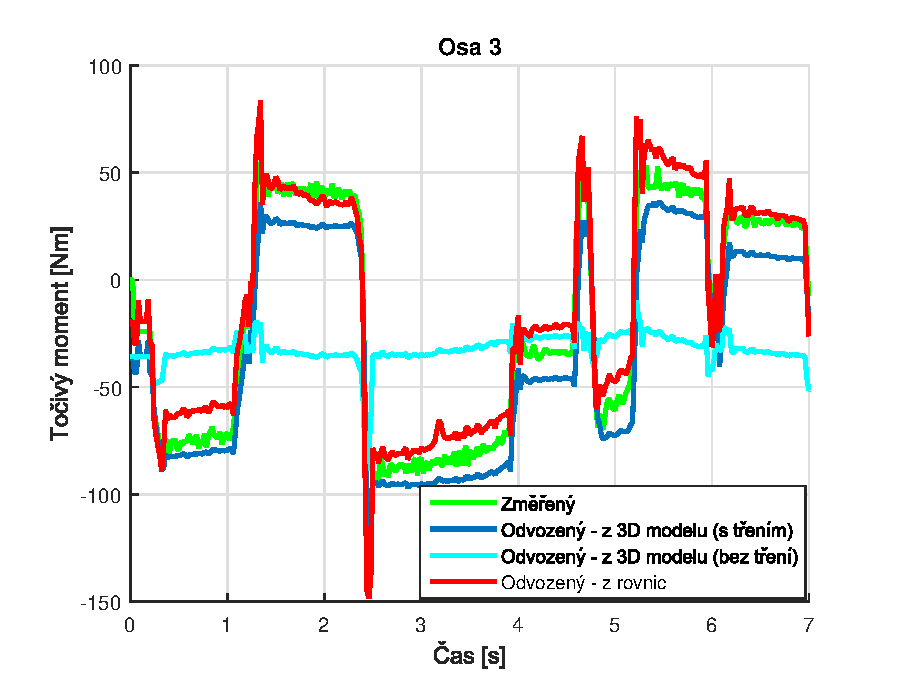
\includegraphics[width=\textwidth]{Osa_3_sim}
        \caption{Osa 3}
        \label{osa_3_sim_pic}
    \end{subfigure}
\end{figure}
\begin{figure}\ContinuedFloat
    \begin{subfigure}[b]{1\textwidth}
        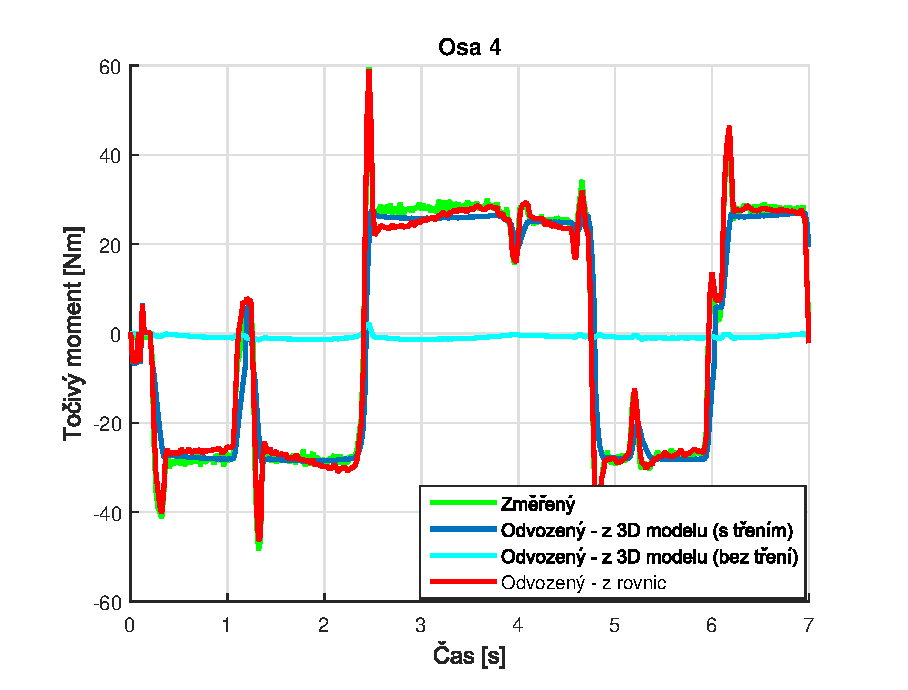
\includegraphics[width=\textwidth]{Osa_4_sim}
        \caption{Osa 4}
        \label{osa_4_sim_pic}
    \end{subfigure}
    \begin{subfigure}[b]{1\textwidth}
        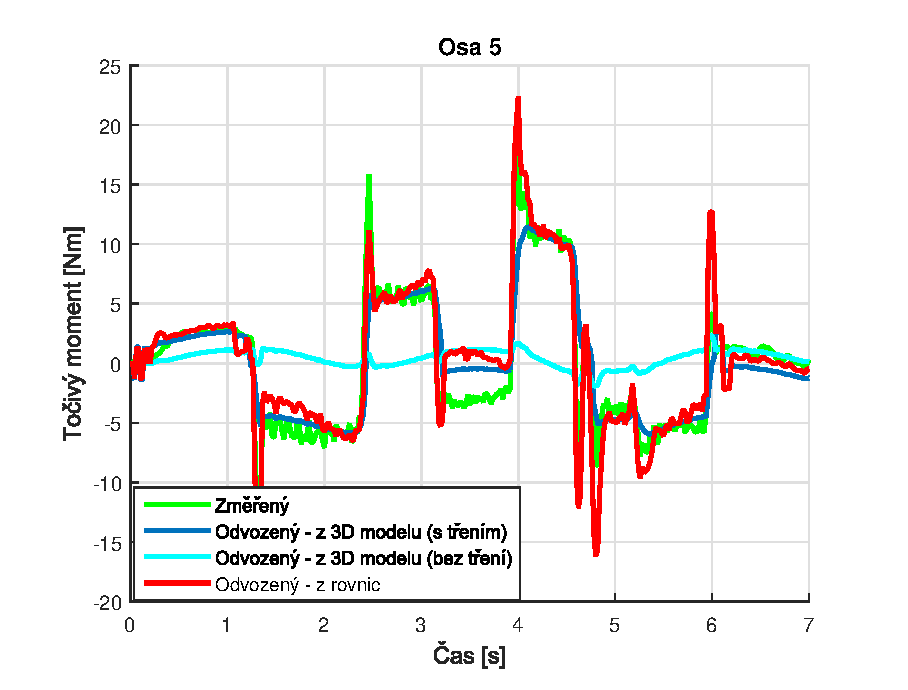
\includegraphics[width=\textwidth]{Osa_5_sim}
        \caption{Osa 5}
        \label{osa_5_sim_pic}
    \end{subfigure}
\end{figure}

\clearpage

\begin{figure}\ContinuedFloat
    \begin{subfigure}[b]{1\textwidth}
        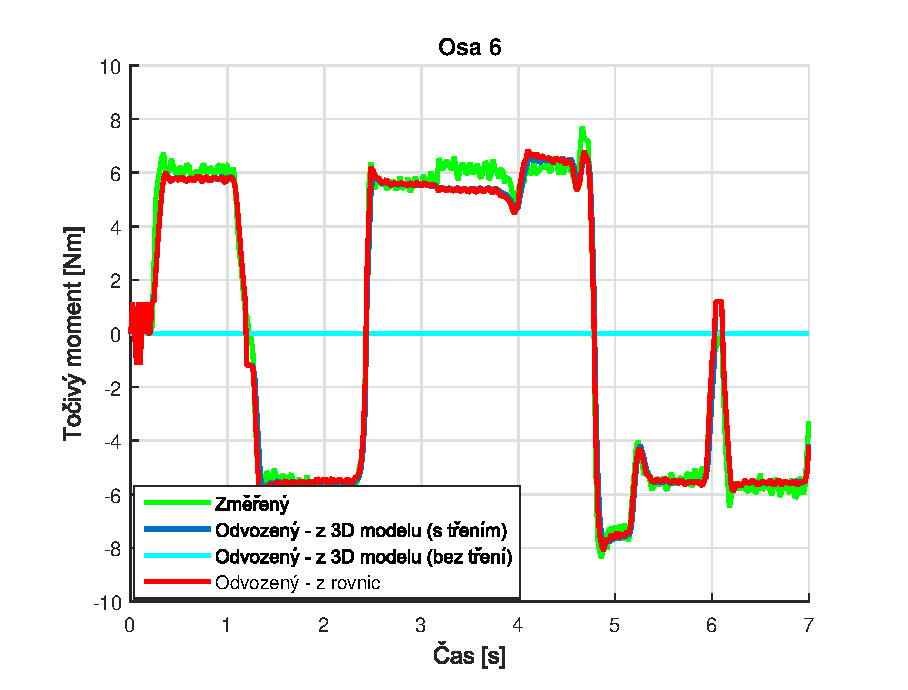
\includegraphics[width=\textwidth]{Osa_6_sim}
        \caption{Osa 6}
        \label{osa_6_sim_pic}
    \end{subfigure}
    \caption{Srovnání měření se simulacemi s odvozenými parametry}\label{osy_sim_pic}
\end{figure}

Z výše uvedených průběhů je patrné, že vypočítané a naměření průběhy si poměrně odpovídají. Ve všech případech se průměrná odchylka pohybuje kolem jedné desetiny Nm a maximální okamžitá odchylka nepřesahuje šest desetin Nm. 

\clearpage

\begin{figure}[h]
    \centering
    \begin{subfigure}[b]{0.49\textwidth}
        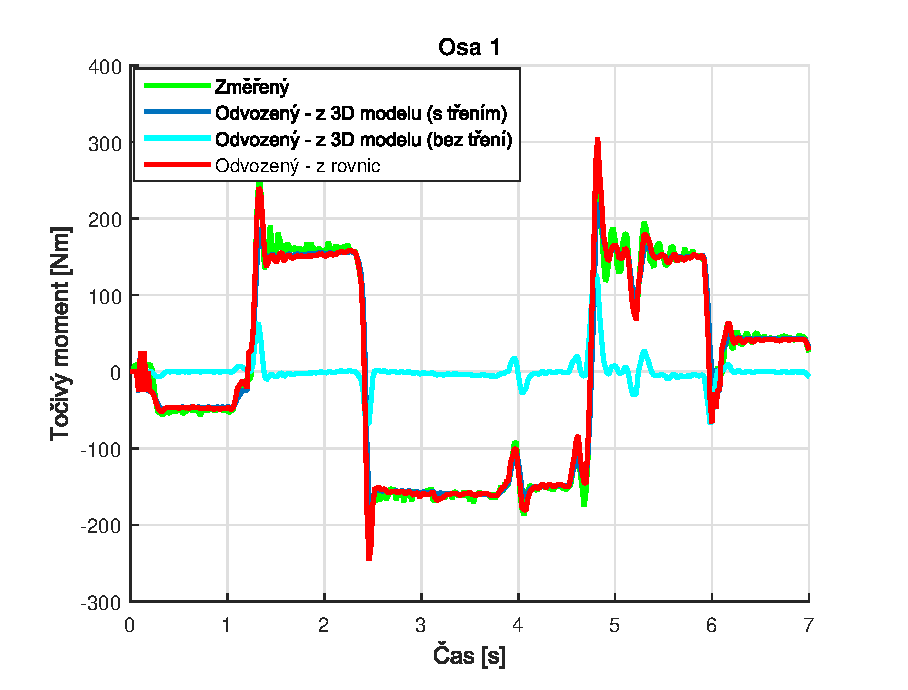
\includegraphics[width=\textwidth]{Osa_1_sim}
        \caption{Osa 1}
        \label{osa_1_sim_pic}
    \end{subfigure}
    \begin{subfigure}[b]{0.49\textwidth}
        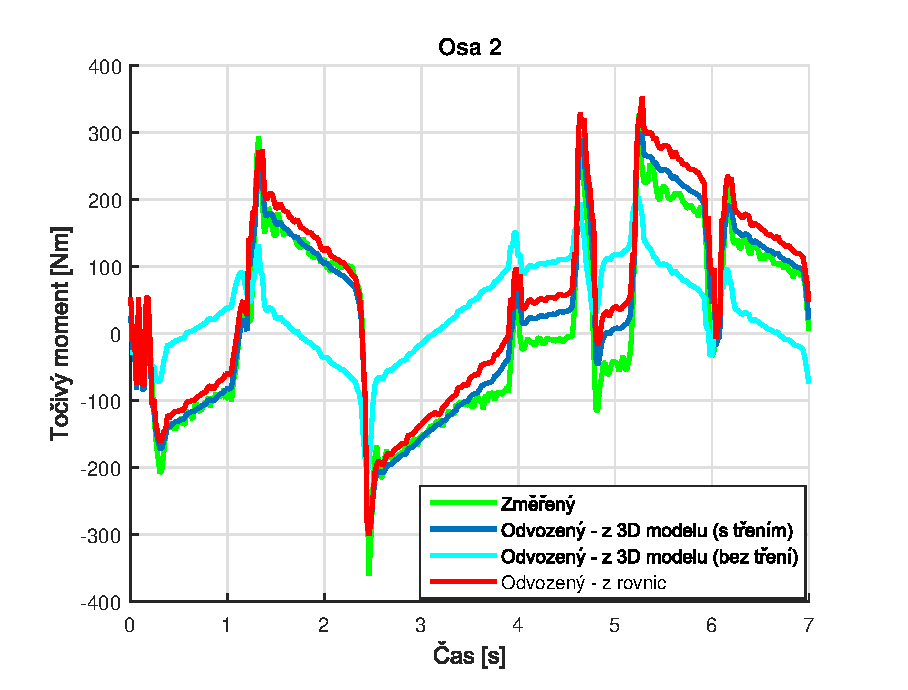
\includegraphics[width=\textwidth]{Osa_2_sim}
        \caption{Osa 2}
        \label{osa_2_sim_pic}
    \end{subfigure}
    \begin{subfigure}[b]{0.49\textwidth}
        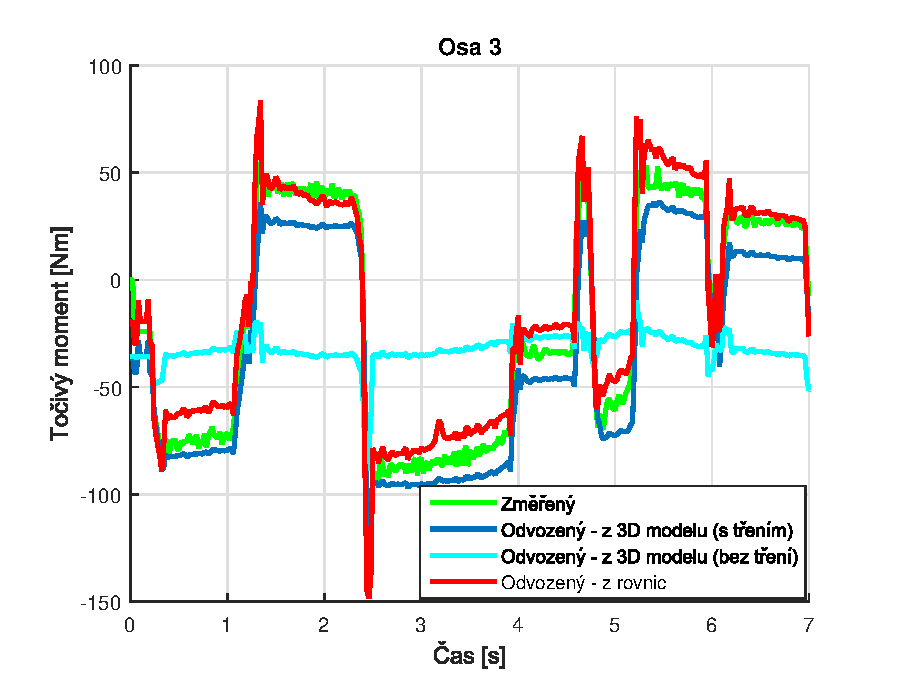
\includegraphics[width=\textwidth]{Osa_3_sim}
        \caption{Osa 3}
        \label{osa_3_sim_pic}
    \end{subfigure}
    \begin{subfigure}[b]{0.49\textwidth}
        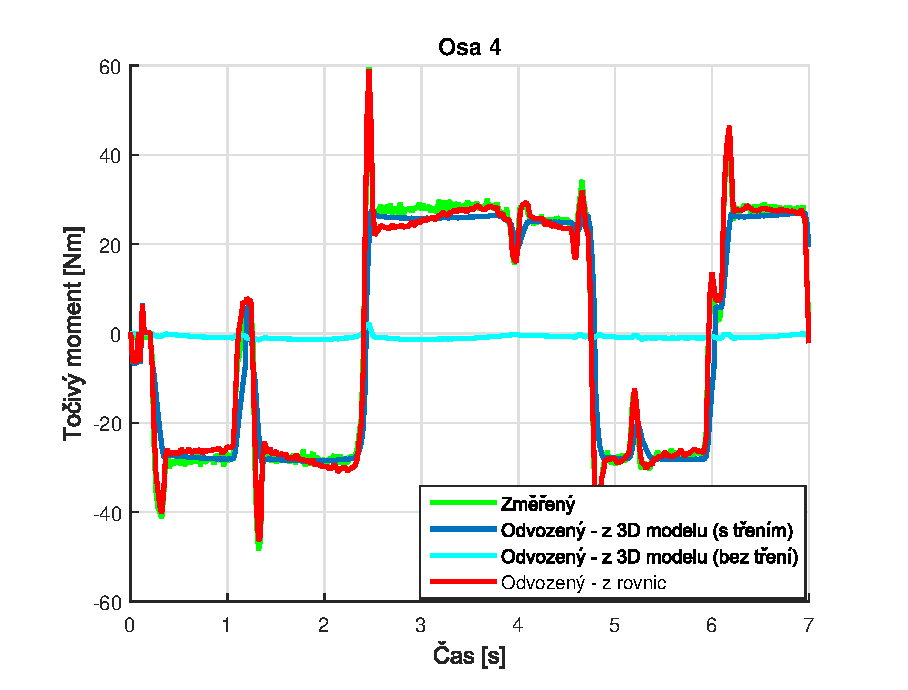
\includegraphics[width=\textwidth]{Osa_4_sim}
        \caption{Osa 4}
        \label{osa_4_sim_pic}
    \end{subfigure}
    \begin{subfigure}[b]{0.49\textwidth}
        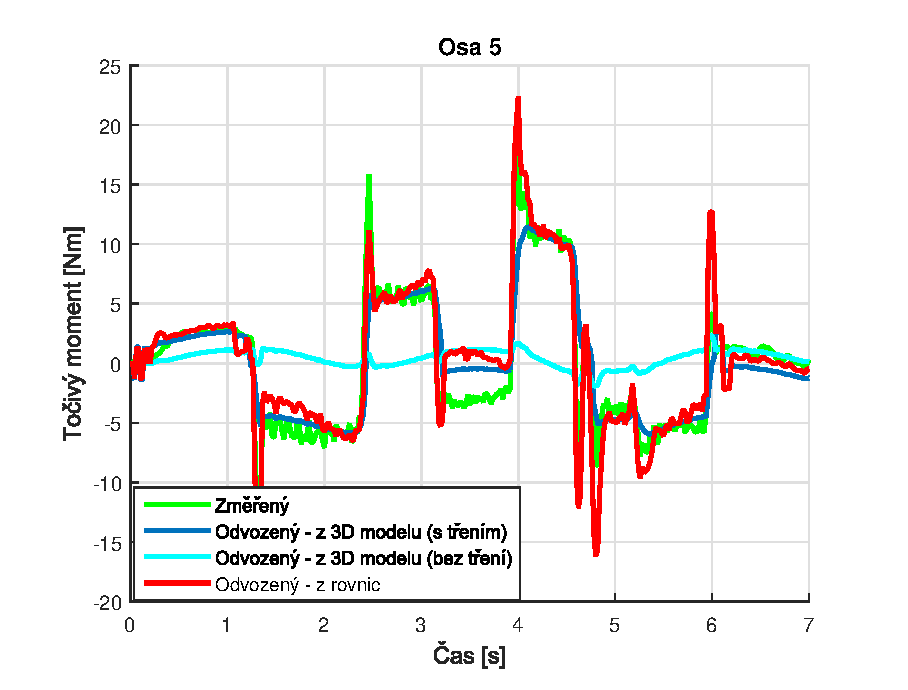
\includegraphics[width=\textwidth]{Osa_5_sim}
        \caption{Osa 5}
        \label{osa_5_sim_pic}
    \end{subfigure}
    \begin{subfigure}[b]{0.49\textwidth}
        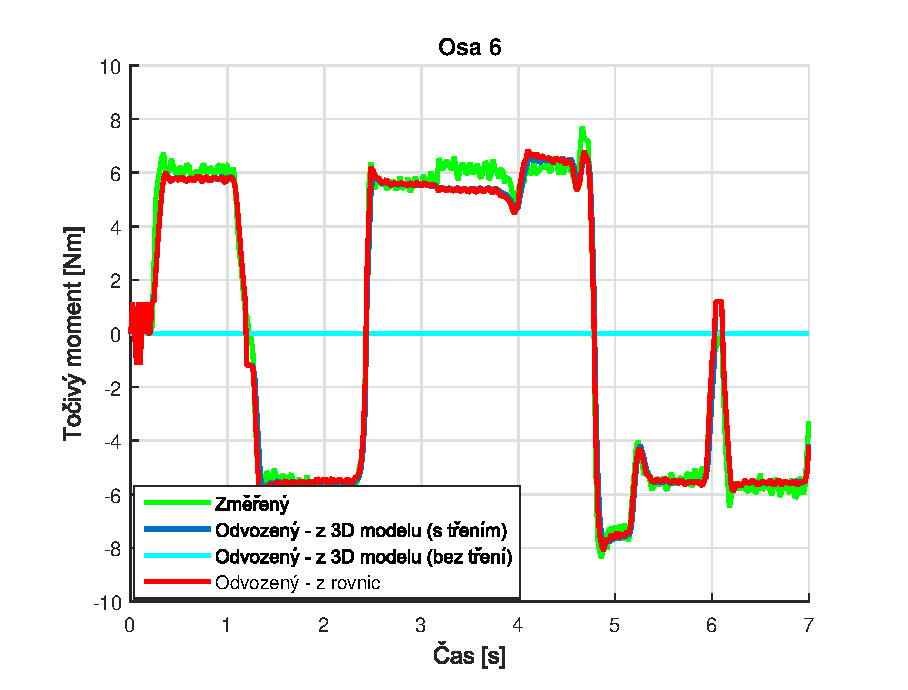
\includegraphics[width=\textwidth]{Osa_6_sim}
        \caption{Osa 6}
        \label{osa_6_sim_pic}
    \end{subfigure}
    \caption{Srovnání měření se simulacemi s odvozenými parametry}\label{osy_sim_pic}
\end{figure}
\chapter{Měření elektrického výkonu}
\label{mereni_el_vykonu_sec}
Správnost odvozeného a identifikovaného modelu robota je potřeba ověřit a porovnat se skutečným měřením elektrického výkonu. 

Měření je prováděno dvěma způsoby. První způsob je měření proudu protékajícího vinutím jednotlivých motorů pomocí nástroje TRACE řídicího systému robotu. Z tohoto měřeného proudu je poté vypočítán elektrický výkon jednotlivých motorů. Druhý způsob je měření skutečného spotřebovaného výkonu celého robotického systému.    

Měření reálného spotřebovaného výkonu bylo provedeno podle schématu na obrázku \ref{schema_mereni_vykonu_pic}. Měřicí sestava je připojena na svorky napájecího vedení mezi elektrickou zásuvkou a skříní s řídicím systémem a napájením robota. Sestava je tvořena měřicí kartou WAGO-I/O-SYSTEM 750 připojenou k průmyslovému PLC Siemens S7-300 CPU 315-2PN/DP. Měřicí karta WAGO obsahuje svorky pro měření napětí a proudu v třífázové síti. 

\begin{figure}[ht]
\includegraphics[width=0.9\textwidth]{mereni_vykonu_obr}
\caption{Schéma zapojení soustavy pro měření výkonu.}
\label{schema_mereni_vykonu_pic}
\end{figure}

Pro účely měření výkonu robotu KUKA KR5 Arc byla karta nakonfigurována pro měření činného výkonu na každé jednotlivé fázi zvlášť. Výsledný celkový výkon je poté podle vzorce \eqref{3ph_power_eq} roven součtu výkonů všech jednotlivých fází. Měření výkonu je prováděno s přesností na desetiny wattu. Vzorkovací perioda měření je 40 ms. 

\section{Měřicí karta WAGO-I/O-SYSTEM 750}

Měřicí karta WAGO-I/O-SYSTEM 750 \cite{wago} je určena pro měření elektrických veličin v třífázové síti. Je navržena pro použití v průmyslovém prostředí v kombinaci s průmyslovým počítačem PLC. 

Karta je opatřena svorkami pro měření napětí a proudu na každé fázi zvlášť. Měření proudu je prováděno pomocí proudového transformátoru převádějícího měřený proud na napětí. 

Kartu je možné nakonfigurovat pro současné měření až čtyř elektrických veličin jako je stejnosměrné (DC) a střídané (AC) napětí, proud, výkon, frekvence, fázový posuv a další, a to pro každou fázi zvlášť. Navíc je karta schopna provádět analýzu harmonických složek signálu pro vybranou fázi a to až pro 3 vybrané harmonické složky z rozsahu 1. a 41. harmonické. 

\begin{figure}[ht]
    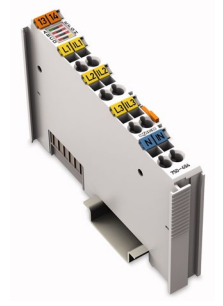
\includegraphics[width=0.3\textwidth]{wago_obr}
    \caption{Měřicí karta WAGO-I/O-SYSTEM 750.}
    \label{wago_pic}
\end{figure}

Změřené veličiny posílá karta přímo na vstupy připojeného PLC, které je dále zpracovává. Měřicí karta se vstupními svorkami je na obrázku \ref{wago_pic}. Technické parametry a podrobnější informace o použití karty je možné nalézt v jejím manuálu \cite{wago}.

\section{PLC Siemens S7-300}

Průmyslové PLC Siemens S7-300 CPU 315-2PN/DP \cite{siemens_plc} zpracovává změřená data, která jsou posílána kartou WAGO 750. PLC tato data cyklicky čte ze vstupů a převádí je do 32-bitového hexadecimálního tvaru. Následně jsou 32-bitová data rozdělena na horních a spodních 16 bitů a opatřena identifikátory. 

Všechna přečtená data s příslušnými identifikátory jsou poté spojena do jedné zprávy, která je navíc ještě opatřena časovou známkou udávající čas o tom, kdy byla data vytvořena. Celá zpráva je nakonec odeslána jako jeden paket pomocí protokolu UDP v síti Profinet.  

Kompletní měřicí systém a program pro sběr měřených dat a jejich odesílání v síti Profinet byl vytvořen Ing. Vojtěchem Pavlíkem v rámci jeho diplomové práce \cite{vojtech_pavlik}. 

Programování a konfigurace PLC je prováděna pomocí nástroje TIA Portal společnosti SIEMENS. Podrobné informace k PLC S7-300 jsou k dispozici v jeho dokumentaci \cite{siemens_plc}.  

\section{Aplikace DEPO} 
\label{aplikacedepo}
Za účelem ukládání změřených dat byla panem Ondřejem Fialou vytvořena aplikace DEPO. Aplikace je napsaná ve skriptovacím programovacím jazyce RUBY. Spouští se pomocí příkazového řádku na osobním počítači připojeném k Ethernetové síti, ke které je připojeno i měřicí PLC. 

Aplikace přijímá data odesílaná měřicím PLC přes protokol UDP. Přijatá data se poté ukládají jako dokument do databáze MongoDB, ke které je počítač připojený. Uložená data v databázi je poté možné exportovat a následně analyzovat.

Pro správnou funkci aplikace je nutné správně nastavit adresu IP měřícího PLC a číslo portu, na kterém má aplikace odesílaná data číst. Nastavení funkčnosti aplikace DEPO se provádí pomocí konfiguračního souboru. Ten obsahuje informace o IP adrese a portu na kterém má data přijímat a dále adresu, název a kolekci databáze, do které se mají data ukládat.

\begin{figure}[ht]
\includegraphics[width=1\textwidth]{schema_mereni}
\caption{Diagram zpracování dat měření výkonu.}
\label{schema_mereni_pic}
\end{figure}

Protože je aplikace napsaná v interpretovaném skriptovacím jazyce RUBY, je možné jí spouštět na libovolném operačním systému, který podporuje spouštění RUBY skriptů. 

Diagram zpracování dat měření výkonu je zobrazen na obrázku \ref{schema_mereni_pic}.


\chapter{Srovnání výsledků}

Odvozený model identifikovaný z rovnic v kapitole \ref{identifikovane_parametry_ch} dává do vztahu točivé momenty s polohami, úhlovými rychlostmi a úhlovými zrychleními na jednotlivých osách (rovnice \ref{celkova_dyn_rovnice_eq}). Tento model je dále možné použít k výpočtu celkového elektrického výkonu robota (viz sekce \ref{el_vykon_ch}).

Vypočítané momenty sil na jednotlivých osách se pomocí momentových konstant převedly na efektivní hodnoty proudů protékajících vinutími motorů. Nahrazením vinutí motorů obvodem s odporem a indukčností zapojenými v sérii byly z těchto hodnot proudů vypočítány jednotlivé hodnoty efektivního napětí na svorkách motorů. Vynásobením hodnot napětí a proudů byly vypočítány elektrické výkony na jednotlivých osách. Celkový elektrický výkon robota je poté dán součtem všech dílčích výkonů na všech osách. 

Pro porovnání modelu pro výpočet výkonu s reálnými naměřenými hodnotami byla použita jiná trajektorie, než která byla použita pro jeho identifikaci. Tato testovací trajektorie byla vytvořena tak, aby se co nejvíce blížila typickým trajektoriím vyskytujícím se v průmyslových aplikacích. Byla vybrána trajektorie simulující montáž součástky A na povrch součástky B. Koncový efektor robota nejprve dojel z výchozí pozice na pozici, kde by se měl vyskytovat zásobník se součástkou A. Poté koncový efektor po obloukové trajektorii dojel na místo montáže součástky A a natočil se do požadovaného úhlu. Následně se vrátil zpět do výchozí pozice.

Při tomto pohybu robota byl v řídícím systému robota spuštěn nástroj TRACE zaznamenávající průběh poloh, úhlových rychlostí a úhlových zrychlení potřebný pro model výkonu. Zároveň bylo spuštěno měřicí PLC ukládající naměřený výkon na napájecím vedení robota. 

\section{Dosažitelná přesnost}

Pro účely srovnání bylo v nástroji TRACE nastaveno i měření efektivních proudů protékajících vinutími motorů na jednotlivých osách. Momenty sil na jednotlivých osách v jsou nástroji TRACE vypočítány ze změřených proudů, podle vzorce \ref{torque_current_eq}, jejich vynásobením příslušnými momentovými konstantami. Proto v případě, že by byly parametry modelu identifikovány naprosto přesně, byl by průběh výkonu vypočítaný pomocí tohoto modelu totožný s výkonem vypočítaným z měření proudů. Výkon spočítaný pomocí těchto změřených proudů představuje maximální možnou hranici přesnosti, které je možné pomocí modelu dosáhnout. 

\begin{figure}[ht]
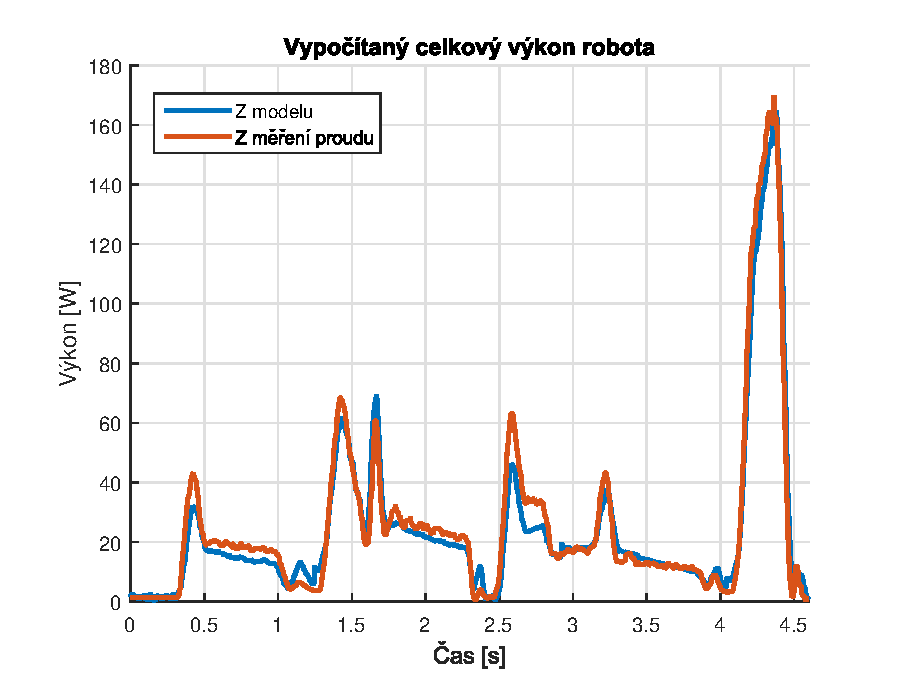
\includegraphics[width=0.90\textwidth]{model_vs_trace}
\caption{Srovnání vypočítaného výkonu z modelu a z měření proudu}
\label{model_vs_trace_pic}
\end{figure}

Na obrázku \ref{model_vs_trace_pic} je zobrazen průběh výkonu vypočítaného z modelu a z přímého měření proudů pomocí nástroje TRACE. Je patrné, že si oba průběhy poměrně odpovídají. Střední odchylka mezi oběma průběhy je 4,86 W. Přesnost odvozeného modelu se tedy blíží maximální možné dosažitelné přesnosti modelování a identifikace z rovnic.

\section{Reálný výkon}


\chapter{Vliv odchylek v parametrech}

Pro vytvoření modelu spotřeby elektrické energie průmyslového robota je potřeba identifikovat mnoho neznámých parametrů. V případě robota KUKA KR5 Arc se jedná o celkem 54 neznámých parametrů. Ne všechny parametry ale ovlivňují dynamiku robota a s ní spojenou spotřebu elektrické energie stejně. Některé parametry mají mnohem větší vliv než jiné. Pro vytvoření co nejpřesnějšího modelu je proto vhodné tyto parametry identifikovat co nejpřesněji. 

V této sekci je provedena analýza vlivu odchylek v jednotlivých identifikovaných parametrech na přesnost modelu. Dynamický model robota je velmi nelineární. Proto není pro analýzu odchylek parametrů možné použít žádnou z lineárních metod, jako je například určení přenosu ze změny parametru na výstupní výkon nebo simulace systému s jednoduchým zvětšením/zmenšením parametrů. 

Z tohoto důvodu je analýza vlivu odchylek v hodnotách parametrů na přesnost energetického modelu robotu provedena použitím metody Monte Carlo. 

\section{Metoda Monte Carlo}

Metody Monte Carlo jsou založeny na vykonání mnoha opakovaných experimentů nebo simulací s náhodně generovanými vstupními parametry za účelem získání numerických výsledků [\cite{monte_carlo_ref}]. Obdrženou sadu výsledků je poté možné analyzovat analytickými nebo stochastickými metodami. Základní myšlenkou metod Monte Carlo je použití nahodilosti k řešení problémů, které mohou být v principu deterministické.

Tyto metody jsou používány k řešení problémů, u kterých je obtížné nebo dokonce nemožné požít některou z analytických metod. Nejčastěji jsou tyto metody používány pro simulace systémů s mnoha stupni volnosti (kapaliny, systémy s rozprostřenými parametry, propojené systémy), výpočet vícerozměrných určitých integrálů, vyhodnocování rizik v ekonomii a mnoho dalších. 

Analýza vlivu odchylek v identifikovaných parametrech pomocí metody Monte Carlo byla provedena tak, že ke každému z identifikovaných parametrů $P_i$ byla náhodně přičtena hodnota z rozsahu $p \in [-P_i,P_i]$, se kterou byla provedena simulace a vypočítaná střední odchylka mezi simulací a změřenými průběhy. Pro každý parametr bylo takto provedeno 200 simulací, pokaždé s náhodně vygenerovanou hodnotou. Ostatní hodnoty parametrů zůstaly nezměněné. 

Po vykonání simulací pro všechny parametry bylo vyhodnoceno, při jakých odchylkách parametrů byl největší rozdíl mezi simulovaným a změřeným průběhem. 

\section{Vyhodnocení}

Vyhodnocené maximální odchylky mezi simulacemi a změřenými průběhy jsou uvedeny v tabulce \ref{tab_odch_parametru}. Hodnoty v tabulce jsou vztaženy ke střední odchylce mezi výkonem vypočítaným pomocí identifikovaného modelu a určeným pomocí měření proudů (viz sekce \ref{dosaz_presnost_sec}). Hodnoty udávají, o kolik se zvýší odchylka ve wattech mezi modelem a měřením vůči původnímu identifikovanému modelu.

\begin{table}[htbp]
  \centering
  \caption{Tabulka maximálních dosažených odchylek vzhledem k odchylkám v parametrech}
    \begin{tabular}{c|cccccccccc}
    \multicolumn{1}{c|}{Osa} & \multicolumn{1}{c}{$I_{xx}$} & \multicolumn{1}{c}{$I_{yy}$} & \multicolumn{1}{c}{$I_{zz}$} & \multicolumn{1}{c}{$d_x$} & \multicolumn{1}{c}{$d_y$} & \multicolumn{1}{c}{$d_z$} & \multicolumn{1}{c}{$m$} & \multicolumn{1}{c}{$f_v$} & \multicolumn{1}{c}{$f_c$} \\
    \hline
    1  & 0     & 0     & 0.349 & 0     & 0     & 0     & 0     & 18.960 & 0.612 \\
    2  & 0.004 & 0.046 & 0.319 & 1.016 & 0.103 & 0     & 0.022 & 17.824 & 0.506 \\
    3  & 0.003 & 0.171 & 0.726 & 2.320 & 0.824 & 0.087 & 8.202 &  0.568 & 0.053 \\
    4  & 0.811 & 0.043 & 0.041 & 0.586 & 0.055 & 0.047 & 7.963 &  0.094 & 0.002 \\
    5  & 0.033 & 0.018 & 0.029 & 0.427 & 0.004 & 0.044 & 1.394 &  0.078 & 0.021 \\
    6  & 0.065 & 0.027 & 0.002 & 0     & 0     & 0.016 & 0.250 &  0     & 0     \\
    \end{tabular}%
  \label{tab_odch_parametru}%
\end{table}%

Z hodnot v tabulce je možné vypozorovat, že největší vliv na přesnost modelu mají koeficienty viskózního tření ($f_v$) osy 1 a 2 a hmotnosti ramen ($m$) os 3 a 4. Na obrázcích \ref{vliv_odch_1} až \ref{vliv_odch_4} jsou znázorněny vlivy jednotlivých odchylek těchto parametrů na celkovou odchylku modelu vůči měření. Na svislé ose je odchylka, o kterou se zvýší střední odchylka modelu vůči měření v závislosti na změně parametru. Na vodorovné ose je pak odchylka v identifikovaném parametru. 

\begin{figure}[h]
    \centering
    \begin{subfigure}[b]{1\textwidth}
        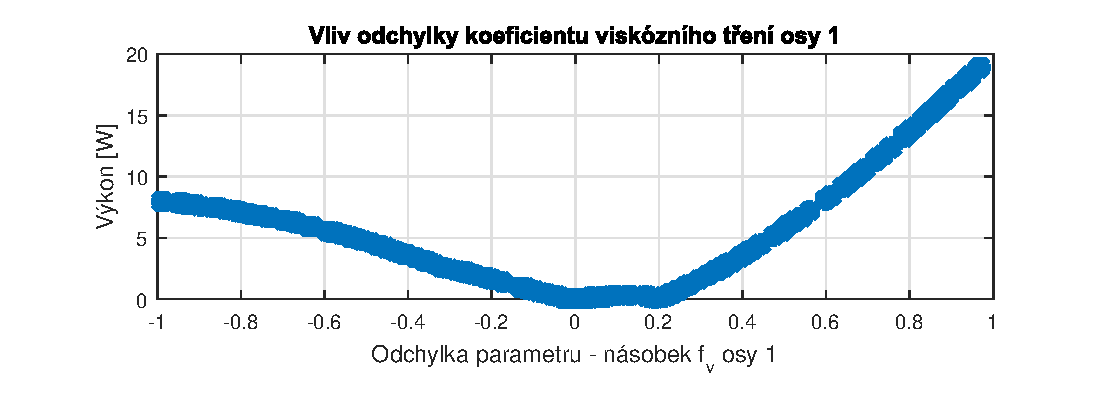
\includegraphics[width=\textwidth]{vliv_odch_osa1_fv}
        \caption{Koeficient viskózního tření osy 1}
        \label{vliv_odch_1}
    \end{subfigure}
    \begin{subfigure}[b]{1\textwidth}
        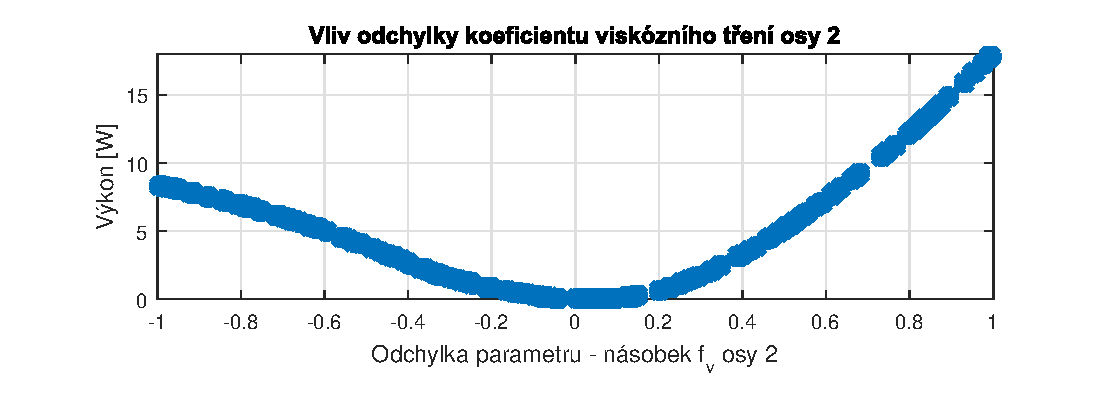
\includegraphics[width=\textwidth]{vliv_odch_osa2_fv}
        \caption{Koeficient viskózního tření osy 2}
        \label{vliv_odch_2}
    \end{subfigure}
    \begin{subfigure}[b]{1\textwidth}
        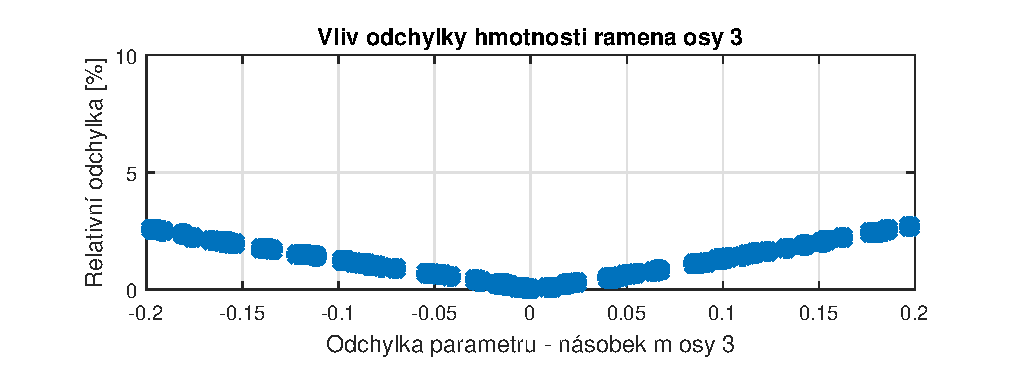
\includegraphics[width=\textwidth]{vliv_odch_osa3_m}
        \caption{Hmotnost osy 3}
        \label{vliv_odch_3}
    \end{subfigure}
    \begin{subfigure}[b]{1\textwidth}
        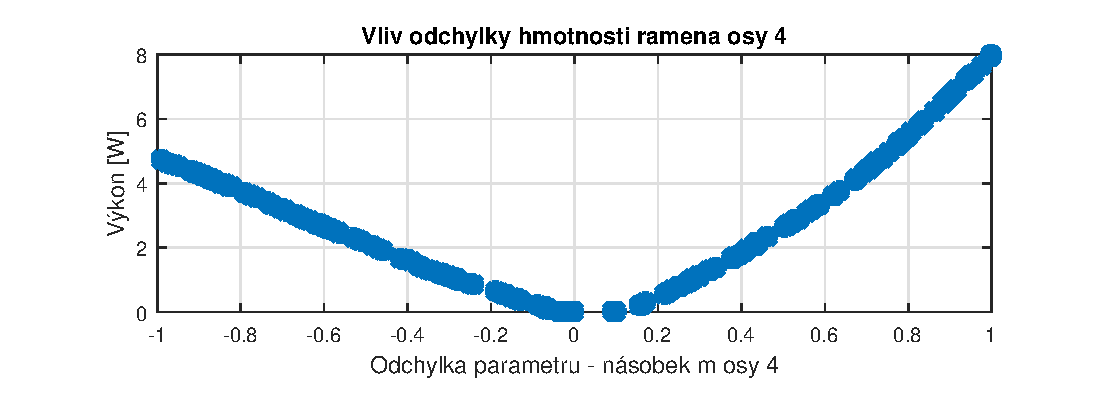
\includegraphics[width=\textwidth]{vliv_odch_osa4_m}
        \caption{Hmotnost osy 4}
        \label{vliv_odch_4}
    \end{subfigure}
    \caption{Vliv odchylek vybraných parametrů na přesnost modelu}
\end{figure} 

\clearpage

Z obrázků je patrné, že metoda identifikace parametrů (viz sekce \ref{z_rovnic_sec}) nalezla optimální řešení, protože zvýšení i snížení identifikovaných parametrů vede na větší střední odchylku mezi modelem a měřením. 

Největší vliv na přesnost modelu mají tedy koeficienty tření, hmotnosti a polohy těžišť prvních tří os. Z toho důvodu je vhodné identifikovat tyto parametry co nejpřesněji.   
\chapter{program}
\chapter{Závěr}

\section{Výsledky práce}

\section{Práce do budoucna}


%\part{Your Party}

%\blindmathtrue

%\blinddocument

%\begin{table}
%\begin{ctucolortab}
%\begin{tabular}{cc}
%\bfseries Foo & \bfseries Bar \\\Midrule
%foo1 & bar1 \\
%foo2 & bar2
%\end{tabular}
%\end{ctucolortab}
%\caption{Foobar.}
%\label{tab:foobar}
%\end{table}

%\begin{figure}
%
\includegraphics[width=0.4\textwidth]{ctu_logo_black}
%\caption{Black logo of the CTU in Pragueueue.}
%\end{figure}

%\begin{figure}[!t]
%
\includegraphics[width=0.4\textwidth]{ctu_logo_blue}
%\caption{Blue logo of the CTU in Pragueueue.}
%\end{figure}

%\chapter{Conclusions}

%\section{Test --- this is just a little test of something in the table of contents}

%\subsection{Yes, table of contents}

%\begin{theorem}\begin{enumerate} \item Bla \item Blo \end{enumerate} \end{theorem}


\medskip

%\begin{proof}\begin{enumerate} \item[8] Bla \item Blo \end{enumerate} \end{proof}

%\appendix

%\printindex

%\appendix

\bibliographystyle{abbrvnat}
\renewcommand{\bibname}{Reference}
\bibliography{ctutest}

%\ctutemplate{specification.as.chapter}

\end{document}